\documentclass[a4paper,12pt,twoside]{memoir}


% Castellano
\usepackage[spanish,es-tabla]{babel}
\selectlanguage{spanish}
\usepackage[utf8]{inputenc}
\usepackage[T1]{fontenc}
\usepackage{lmodern} % Scalable font
\usepackage{microtype}
\usepackage{placeins}
\usepackage{listings}

\usepackage[style=numeric,sorting=none]{biblatex} % Para la bibliografia
\addbibresource{bibliografia.bib} % Para la bibliografia
\usepackage{geometry} 

\RequirePackage{booktabs}
\RequirePackage[table]{xcolor}
\RequirePackage{xtab}
\RequirePackage{multirow}

% Links
\PassOptionsToPackage{hyphens}{url}\usepackage[colorlinks]{hyperref}
\hypersetup{
	allcolors = {black} % Quitar o volver a poner a 'red' o 'black'
}

% Ecuaciones
\usepackage{amsmath}

% Rutas de fichero / paquete
\newcommand{\ruta}[1]{{\sffamily #1}}

% Párrafos
\nonzeroparskip

% Huérfanas y viudas
\widowpenalty100000
\clubpenalty100000

\let\tmp\oddsidemargin
\let\oddsidemargin\evensidemargin
\let\evensidemargin\tmp
\reversemarginpar

% Imágenes

% Comando para insertar una imagen en un lugar concreto.
% Los parámetros son:
% 1 --> Ruta absoluta/relativa de la figura
% 2 --> Texto a pie de figura
% 3 --> Tamaño en tanto por uno relativo al ancho de página
\usepackage{graphicx}

\newcommand{\imagen}[3]{
	\begin{figure}[!h]
		\centering
		\includegraphics[width=#3\textwidth]{#1}
		\caption{#2}\label{fig:#1}
	\end{figure}
	\FloatBarrier
}







\graphicspath{ {./img/} }

% Capítulos
\chapterstyle{bianchi}
\newcommand{\capitulo}[2]{
	\setcounter{chapter}{#1}
	\setcounter{section}{0}
	\setcounter{figure}{0}
	\setcounter{table}{0}
	\chapter*{#2}
	\addcontentsline{toc}{chapter}{#2}
	\markboth{#2}{#2}
}

% Apéndices
\renewcommand{\appendixname}{Apéndice}
\renewcommand*\cftappendixname{\appendixname}

\newcommand{\apendice}[1]{
	%\renewcommand{\thechapter}{A}
	\chapter{#1}
}

\renewcommand*\cftappendixname{\appendixname\ }

% Formato de portada

\makeatletter
\usepackage{xcolor}
\newcommand{\tutor}[1]{\def\@tutor{#1}}
\newcommand{\tutorb}[1]{\def\@tutorb{#1}}

\newcommand{\course}[1]{\def\@course{#1}}
\definecolor{cpardoBox}{HTML}{E6E6FF}
\def\maketitle{
  \null
  \thispagestyle{empty}
  % Cabecera ----------------
\begin{center}
  \noindent
\includegraphics[width=\textwidth]{cabeceraSalud}\vspace{1.5cm}%
\end{center}
  
  % Título proyecto y escudo salud ----------------
  \begin{center}
    \begin{minipage}[c][1.5cm][c]{.20\textwidth}
        
\includegraphics[width=\textwidth]{escudoSalud.pdf}
    \end{minipage}
  \end{center}
  
  \begin{center}
    \colorbox{cpardoBox}{%
        \begin{minipage}{.8\textwidth}
          \vspace{.5cm}\Large
          \begin{center}
          \textbf{TFG del Grado en Ingeniería de la Salud}\vspace{.6cm}\\
          \textbf{\LARGE\@title{}}
          \end{center}
          \vspace{.2cm}
        \end{minipage}
    }%
  \end{center}
  
    % Datos de alumno, curso y tutores ------------------
  \begin{center}%
  {%
    \noindent\LARGE
    Presentado por \@author{}\\ 
    en la Universidad de Burgos\\
    \vspace{0.5cm}
    \noindent\Large
    \@date{}\\
    \vspace{0.5cm}
    Tutor: \@tutor{}\\ % comenta el que no corresponda
    %Tutores: \@tutor{} -- \@tutorb{}\\
  }%
  \end{center}%
  \null
  \cleardoublepage
  }
\makeatother

\newcommand{\nombre}{Naiara Gadea Rodríguez Gómez}
\newcommand{\nombreTutor}{Pedro Luis Sánchez Ortega} 
\newcommand{\nombreTutorb}{Tutor 2} 
\newcommand{\dni}{71755517W} 

% Datos de portada
\title{Título del trabajo}
\author{\nombre}
\tutor{\nombreTutor}
\tutorb{\nombreTutorb}
\date{\today}


\begin{document}

\maketitle


\newpage\null\thispagestyle{empty}\newpage

%%%%%%%%%%%%%%%%%%%%%%%%%%%%%%%%%%%%%%%%%%%%%%%%%%%%%%%%%%%%%%%%%%%%%%%%%%%%%%%%%%%%%%%%
\thispagestyle{empty}


\noindent
\includegraphics[width=\textwidth]{cabeceraSalud}\vspace{1cm}

\noindent D. \nombreTutor, profesor del departamento \textcolor{red}{de departamento}, área de \textcolor{red}{área}.

\noindent Expone:

\noindent Que el alumno D. \nombre, con DNI \dni, ha realizado el Trabajo final de Grado en Ingeniería de la Salud titulado \textcolor{red}{título del trabajo}. 

\noindent Y que dicho trabajo ha sido realizado por el alumno bajo la dirección del que suscribe, en virtud de lo cual se autoriza su presentación y defensa.

\begin{center} %\large
En Burgos, {\large \today}
\end{center}

\vfill\vfill\vfill

% Author and supervisor
\begin{minipage}{0.45\textwidth}
\begin{flushleft} %\large
Vº. Bº. del Tutor:\\[2cm]
D. \nombreTutor
\end{flushleft}
\end{minipage}
\hfill
%\begin{minipage}{0.45\textwidth}
%\begin{flushleft} %\large
%Vº. Bº. del Tutor:\\[2cm]
%D. \nombreTutorb
%\end{flushleft}
%\end{minipage}
\hfill

\vfill

% para casos con solo un tutor comentar lo anterior
% y descomentar lo siguiente
%Vº. Bº. del Tutor:\\[2cm]
%D. nombre tutor


\newpage\null\thispagestyle{empty}\newpage




\frontmatter

% Abstract en castellano
\renewcommand*\abstractname{Resumen}
\begin{abstract}

Este trabajo se centra en la búsqueda de una solución a una necesidad real con el fin de la búsqueda de un dispositivo de control postural para el apoyo de la mejora de la postura en diferentes colectivos. Durante el desarrollo del proyecto se han estudiado los aspectos teóricos de la postura y el control postural. Por otro lado, se ha indagado en las distintas soluciones disponibles en el mercado actual con el fin de predefinir las características básicas que debería tener el dispositivo ideado. 

Tras la obtención de la idea, se ha realizado una búsqueda de los posibles componentes y se han sopesado los componentes a incluir. Se han creado dos versiones del prototipo. En la primera versión se emplea un sensor de inclinación muy sencillo y en la segunda versión se utiliza un sensor MPU más complejo que ofrece más precisión y mayores posibilidades. En el proyecto también se propone un prototipo de interfaz de una aplicación de interacción usuario-dispositivo.

La última versión del prototipo consigue un correcto control postural. Sin embargo, al tratarse de un prototipo, existen varios puntos de mejora y en el proyecto se ofrecen diferentes líneas para seguir el proyecto en un futuro.

\end{abstract}

\renewcommand*\abstractname{Descriptores}
\begin{abstract}

Control postural, postura, prototipo, dispositivo, ayuda, aplicación, aplicación interactiva, autonomía, estudio del arte, mejora, necesidad, solución, accesibilidad, sencillez, bajo coste...

\end{abstract}

\clearpage

% Abstract en inglés
\renewcommand*\abstractname{Abstract}
\begin{abstract}
This work focuses on finding a solution to a real need in order to find a postural control device to support posture improvement in different groups. During the development of the project, the theoretical aspects of posture and postural control were studied. On the other hand, we have investigated the different solutions available in the current market in order to specify the basic features that the device should have. 

After obtaining the idea, a search of the possible components was made and the components to be incuded were weighed. Two versions of the prototype have been created. The first version uses a very simple tilt sensor and the second version uses a more complex MPU sensor that offers more precision and greater possibilities. The project also proposes a prototype app interface for well user-device interaction.

The latest version of the prototype achieves correct postural control. However, the fact of being a prototype, there are several points of improvement. Different lines have been included to further develop and improve the project in the future.


\end{abstract}

\renewcommand*\abstractname{Keywords}
\begin{abstract}
Postural control, posture, prototype, device, help, application, interactive application, autonomy, art study, improvement, need, solution, accessibility, simplicity, low cost...
\end{abstract}

\clearpage

% Indices
\tableofcontents

\clearpage

\listoffigures

\clearpage

\listoftables
\clearpage


\mainmatter
\capitulo{1}{Objetivos}

Objetivos principales del trabajo realizado.

Este apartado explica de forma precisa y concisa cuales son los objetivos que se persiguen con la realización del proyecto. Se puede distinguir entre:
\begin{enumerate}
    \item Los objetivos marcados por los requisitos del software/hardware/análisis a desarrollar.
    \item Los objetivos de carácter técnico, relativos a la calidad de los resultados, velocidad de ejecución, fiabilidad o similares.
    \item Los objetivos de aprendizaje, relativos a aprender técnicas o herramientas de interés. 
    \item x
    \item Este trabajo tiene como objetivo una busqueda del estado del arte de dispositivos que tienen relación con el control postural y la creación de un dispositivo lo más sencillo y completo posible que sea capaz de identificar y avisar que una persona tiene una buena o mala postura para poder así abordar y mejorar la postura con aprendizaje dinámico.
    
    \item Suponer una ayuda para la Asosciación del Parkinson de Burgos.
    
\end{enumerate}









\capitulo{2}{Introducción}
% Se pueden añadir todas las subsecciones que queramos o necesitemos.

Descripción del contenido del trabajo y de la estructura de la memoria y del resto de materiales entregados.


\section{Conceptos teóricos básicos.} %Explicación de los conceptos teóricos básicos necesarios para que cualquier miembro del tribunal pueda entender el trabajo realizado.
Para llevar a cabo este trabajo hay que comprender su base, en este caso el control postural, qué es, su importancia y todo lo que ello conlleva.\cite{wiki:latex} % Citar el librio

Antes de comenzar se deben conocer los siguientes conceptos básicos y componentes que engloban el control postural:

\begin{itemize}
    \item Centro de masas o CDM que es la media de todos los centros de masas de las distintas partes del cuerpo, es responsable del equilibrio.
    \item Centro de presiones o CDP es la proyección sobre la base de sustentación del centro de masas del cuerpo.
    \item Centro de gravedad o CDG es el punto del cuerpo donde se concentra la fuerza de gravedad.
    \item Área de apoyo es el área sobre la que el cuerpo descarga su peso de forma efectiva.
    \item Base de sustentación que es la superficie disponible sobre la que un cuerpo puede apoyar su peso.
    \item Límite de estabilidad es el trayecto por el cual una persona puede realizar un movimiento sin perder su equilibrio y poder realizar ajustes posturales, este límite no es fijo, depende del tiempo, de la tarea o del entorno.
    \item Postura es la orientación y el alineamiento del cuerpo respecto al entorno.
    \item Orientación postural es la capacidad de mantener la relación entre las distintas partes del cuerpo y el entorno para realizar una actividad.
    \item Sinergia postural es la relación entre la contracción muscular y las rotaciones articulares para estabilizar la postura.
    \item Balanceo postural es el desplazamiento constante y la corrección del centro de gravedad para mantener la postura.
\end{itemize}

La postura nace de la relación entre el entorno, el individuo y la actividad que debe realizar. Y, por tanto, el control postural es el control de la posición corporal en el espacio con el fin de obtener la estabilidad, y la orientación que necesitamos para poder realizar las actividades diarias, su profesión o aficiones. La estabilidad se define como la capacidad de mantener la proyección del centro de gravedad dentro de una base de sustentación, mientras que la orientación es la capacidad de mantener la relación adecuada entre las distintas partes del cuerpo al realizar una tarea teniendo en cuenta el entorno.

Para poder cumplir con el objetivo del control postural el cuerpo tiene que anticiparse, mantenerse y reaccionar. El control postural requiere que interaccionen distintos sistemas del cuerpo para abarcar la estabilidad, la percepción de la orientación espacial, el alineamiento del cuerpo, la lucha contra la gravedad al realizar un movimiento y la respuesta a posibles perturbaciones de origen sensorial o mecánico.

Principalmente en el control postural interviene el sistema nervioso, como centro de control, manteniendo la postura y el equilibrio gracias a la recogida e interpretación de información de los receptores y a la producción de órdenes; y, el sistema musculoesquelético, ya que se requiere de una musculatura capaz de adaptarse a los cambios. Además, se utilizan experiencias previas para elaborar el esquema corporal.

Por todo ello se va a conocer la relación del sistema nervioso y la postura, algunas estrategias del control postural y su importancia o desarrollo.

%Subseccion
\subsection{El sistema nervioso y la postura.} 
El sistema nervioso se compone de diferentes estructuras como son las neuronas o las células de neuroglia que se encargan de mantener la homeostasis corporal regulando y coordinando las distintas funciones del organismo.

Asimismo, el sistema nervioso se puede dividir en sistema nervioso central que se encuentra compuesto por la médula espinal y el encéfalo, y el sistema nervioso periférico que está compuesto por ganglios y nervios.

El sistema nervioso también se puede dividir en función del tipo de respuestas de las que se encargan, si se encarga de las respuestas involuntarios se trata del sistema nervioso autónomo que, a su vez, se divide en los sistemas simpático y parasimpático. En el caso de las respuestas voluntarias del organismo se llama sistema nervioso somático.

Los receptores son los que se encargan de recoger la información que recibe el sistema nervioso mediante mecanismos de retroalimentación, estos elementos se encuentran en los músculos, para poder detectar el movimiento. Por otra parte, se necesita también la información recogida por la vista, el sistema vestibular del oído interno o las señales procedentes de las modificaciones de presión.

Si en algún caso se producen perturbaciones los receptores detectarán esos imprevistos y proporcionarán información acerca de las nuevas condiciones para así adaptar el tono postural. Por ejemplo si los receptores de presión de los pies registran el desplazamiento mínimo durante la bipedestación y se transmite la información por el nervio periférico, seguido de la medula espinal, el tracto espinocerebeloso y desde el cerebelo a la formación reticular y a los núcleos vestibulares. Si se desplaza la cabeza se crea una aceleración en dirección anterior que se registra y se transmite esa información a los núcleos vestibulares. 

Las reacciones de equilibrio son la respuesta al control postural, los núcleos vestibulares activan la musculatura de la core-stability que está formada por los músculos del suelo pélvico, los músculos profundos paravertebrales y sacrolumbares, y, la musculatura abdominal y lateral. En función del tipo de desplazamiento se activarán una cadena u otra, ya sean la cadena anterior, la posterior, la lateral o combinaciones de las mismas.

\subsection{Estrategias de control postural.} 
El control postural y sus ajustes se dan en tronco, tobillos y caderas, para así mantener el equilibrio, creando la estabilidad que permite los movimientos al realizar distintas actividades.

Existe un modelo que define 3 elementos que modifican, construyen y mantienen la postura, el modelo de sistemas dinámicos de Bernstein. Lo elementos en cuestión son los factores individuales, la tarea a realizar y el entorno. 

Los factores individuales son aquellos pertenecientes a cada individuo, pueden variar su influencia con entrenamiento. Dentro de los factores individuales encontramos los elementos sensitivos que dan información respecto al movimiento y la posición del centro de gravedad e incluyen las aferencias visuales (posición respecto al entorno), el sistema somatosensitivo (son los receptores de los músculos, la piel u otros tejidos, dan información acerca de las variaciones de la orientación postural) y el vestibular (es básicamente el oído, posición de la cabeza); también encontramos los elementos motores que hacen referencia a las exigencias musculoesqueléticas (fuerza, flexibilidad o alineación de las partes del cuerpo) y neuromusculares (patrones de movimiento y contracción de los músculos)  necesarias para el ajuste postural; y, los elementos cognitivos que refieren a las necesidades psicológicas y cognitivas relacionadas con la actitud postural.

Igualmente, existen diferentes estrategias de control de la postura, como aquellas que se centran en el equilibrio, controlando las oscilaciones o balanceos espontáneos. Algunas de estas estrategias son las de controlar la correcta alineación corporal, minimizando las fuerzas gravitatorias; el suficiente tono muscular mediante el control de la resistencia de un músculo a ser estirado; el correcto tono postural, a partir del control de la fuerza de gravedad; o, el control de las reacciones posturales o de balance mediante ajustes compuestos de reacciones de equilibrio, enderezamiento y de apoyo. 

Por otro lado, la memoria implícita que se da en el cerebelo y en los núcleos basales proporciona información sobre dónde, cuánto y cómo se debe ajustar el tono postural para compensar los desplazamientos.

Otras estrategias para mantener el control postural son las que describen Shumway-Cook y Woollacott, la ‘ankle strategy’ que se basa en la bipedestación mantenida por la base de sustentación pequeña que serán los tobillos, la ‘hip strategy’ que se basa en controlar los centros de masas en un desplazamiento de peso mayor y la ‘stepping strateging’ que se basa en una base de sustentación aún mayor.

\subsection{Desarrollo del control postural.} 
Las necesidades de estabilidad cambian con la tarea que se debe realizar. El desarrollo de control postural en niños se produce en tres etapas, primero, se debe desarrollar el control encefálico, después la sedestación (capacidad de sentarse) y, por último, la bipedestación.

Además, la postura y el equilibrio varían con la edad, por una parte, los niños pequeños no tienen suficientemente desarrollado las aferencias sensoriales, y por otra los adultos mayores presentan involución cognitiva de sus estructuras cerebrales, todos ellos ven disminuido el control postural.

Asimismo, pacientes con traumatismos craneoencefálico, esclerosis múltiple, infartos u otras lesiones en el sistema nervioso central pueden tener afectado alguno de elementos implicados en el control de la postura y por lo que su control postural se verá afectado. En algunos casos también influyen los factores psicológicos, una persona con depresión o un problema de atención también puede llegar a influir sobre ese control postural.


%Sub-subseccion
\subsubsection{Sub Subsección}

\subsubsection{Sub Subsección}

En esta sección y el resto de secciones de la memoria puede ser necesario incluir listas de items.

% Listas de puntos 
\begin{itemize}
    \item item1
    \item item2
    \item item3
\end{itemize}

Listas enumeradas.
% Enumeraciones
\begin{enumerate}
    \item item1
    \item item2
    \item item3
\end{enumerate}

Figuras, como la figura \ref{fig:escudo} que aparece en la página \pageref{fig:escudo}. 

Puedes aprender más de las figuras en la dirección \url{https://es.overleaf.com/learn/latex/Inserting_Images} % más informacion de como utilizar figuras

% Inicio de la figura
\begin{figure}[h]
    \centering
    
\includegraphics[width=0.25\textwidth]{img/escudoSalud.pdf}
    \caption{Pie de la figura}
    \label{fig:escudo} % Esta etiqueta es la que permite que se encuentr referenciada en el texto (es muy importante que siempre estén referenciadas en el texto)
\end{figure}


También se pueden insertar tablas como \ref{tab:my-table}, que ha sido generada con \url{https://www.tablesgenerator.com/}. % Este enlace permite crear tablas y te genera el código latex

% Ejemplos de tablas
\begin{table}[]
\begin{tabular}{lll}
a & b & c \\
1 & 2 & 3 \\
4 & 5 & 6
\end{tabular}
\caption{}
\label{tab:my-table}
\end{table}

Es necesario que todas las figuras y tablas aparezca referenciadas en el texto, como estos ejemplos.

Todos los conceptos teóricos deben de estar correctamente referenciados en la bibliografía. Por ejemplo, aquí estoy citando la página de \LaTeX{} de Wikipedia \cite{wiki:latex}. %El comando \cite permite referenciar las citas bibliográficas, siempre se tienen que referenciar las citas de la bibliografía.

También puede ser necesario utilizar notas al pie \footnote{como por ejemplo esta}, para aclarar algunos conceptos.


\section{Estado del arte y trabajos relacionados.}

Revisión bibliografica de que se está haciendo en la industria o la academia relativo al problema que se está tratando.

Enumeración y resumen de todos los trabajos relacionados de interés.


\capitulo{3}{Metodología}

\section{Descripción de los datos.}
\textcolor{red}{
Breve descripción de los datos.
En caso de tratarse de un trabajo donde los datos son muy importantes, puede haber explicaciones extra en el anexo correspondiente. yo creo que aquí puedes describir los datos que vas a recoger, sean muchos o pocos. Date cuenta que pocos datos pero de muchísimas personas si son ya una entidad de estudio. 
Pero creo que si es necesario indicar el tipo de datos y su magnitud. Para mostrarlo desde el principio. Puedes también hacer referencia a las unidades de ángulos de rotación o inclinación, aceleraciones en un punto determinado y movimientos }

\textcolor{red}{En este trabajo no se utilizan tablas de datos.}

\textcolor{red}{Nose...}
\textcolor{red}{El dispositivo ideado trabajará con los datos que se obtienen de la monitorización de la postura del usuario, ya se encuentre sentado o de pie, alertando en caso de detección de una postura dañina durante un periodo de tiempo determinado. De esta forma se logrará que se desarrolle una postura natural correcta y, por lo tanto saludable. }

\textcolor{red}{La postura correcta prevendrá de posibles lesiones, u otros daños y el desarrollo correcto de las actividades.}

\textcolor{red}{Se trabajarán con los ángulos de rotación o inclinación, aceleraciones en un punto determinado y movimientos que realiza una persona al modificar su postura. Para detectar una correcta o incorrecta postura se establecerá un umbral donde se considerará que la persona está en una buena postura, por lo que, fuera de ese umbral, la persona tendrá una mala postura y el dispositivo emitirá un aviso para que la persona modifique su postura.}
 
\section{Técnicas y herramientas.}

\textcolor{red}{recuerda indicar para que usas cada una de ellas y porque esa Y no otras (si puede ser)}

\textcolor{red}{Esta parte de la memoria tiene como objetivo presentar las técnicas metodológicas y las herramientas de desarrollo que se han utilizado para llevar a cabo el proyecto. Si se han estudiado diferentes alternativas de metodologías, herramientas, bibliotecas se puede hacer un resumen de los aspectos más destacados de cada alternativa, incluyendo comparativas entre las distintas opciones y una justificación de las elecciones realizadas. }

\textcolor{red}{No se pretende que este apartado se convierta en un capítulo de un libro dedicado a cada una de las alternativas, sino comentar los aspectos más destacados de cada opción, con un repaso somero a los fundamentos esenciales y referencias bibliográficas para que el lector pueda ampliar su conocimiento sobre el tema.}

\textcolor{red}{Añadir los posibles sensores, el cable USB, microcontrolador (En mi caso arduino (hardware y software en C++ simplificado)). Las aplicaciones que se han usado para la realización del proyecto... Se deberá explicar porque se han usado unos sensores u otros (si se hace una tabla comparativa mejor). }

\subsection{Aplicaciones empleadas.}

\begin{itemize}
\item \textbf{Overleaf}\cite{Overleaf}: es un editor LaTeX colaborativo en línea, que se emplea para la creación, edición y publicación de documentos científicos. LaTeX es una herramienta que a partir del procesamiento de un documento de texto plano compuesto por texto y comandos LaTeX por el software de TeX engine convierte los comandos LaTeX y el texto del documento en un archivo PDF profesional. Esta es la herramienta que se ha empleado para la realización de este documento. Se puede acceder a través de https://www.overleaf.com  %(Referencia: https://www.overleaf.com/learn/latex/Learn_LaTeX_in_30_minutes#What_is_LaTeX )

\item \textbf{Diagrams.net}\cite{Diagrams.net}: es una aplicación de código abierto para la realización de diagramas online, con gran cantidad de librerías de formas para su realización. Esta aplicación es la que se ha empleado para la realización de la gran mayoría de diagramas del proyecto y los prototipos de interfaz. Se puede acceder a través de: https://www.diagrams.net % Referencia: https://www.diagrams.net/doc/getting-started-editor  

\item \textbf{Tinkercad}\cite{Tinkercad}:es una aplicación web gratuita que permite desarrollar habilidades de diseño 3D, electrónica y programación, sin necesidad de utilizar ningún tipo de software adicional. En este proyecto se ha empleado esta herramienta para la simulación del diseño del circuito electrónico, ya que permite realizar circuitos y componentes desde 0 o empleando sus circuitos predefinidos. Además, esta aplicación consta de un editor de código que permite programar las simulaciones. Se puede acceder a través de: https://www.tinkercad.com %Referencia: https://www.tinkercad.com/circuits 

\item \textbf{Arduino}\cite{Arduino1, Arduino2}: plataforma de código abierto de electrónica basada en hardware y software simple y accesible, originalmente creada para la creación rápida de prototipos. Existen diferentes placas de Arduino con distintas funciones. Se puede introducir en el microcontrolador un conjunto de instrucciones que se quiere que realice el dispositivo mediante el uso del software de Arduino (IDE), estas instrucciones están escritas en el lenguaje de programación Arduino, que es similar a C++ pero simplificado, además se puede expandir el lenguaje utilizando distintas bibliotecas C++. Esta plataforma es muy utilizada y ha permitido crear gran variedad de proyectos. Su sencillez, accesibilidad y coste son las principales razones por las que se ha pensado en realizar el prototipo de este proyecto basado en esta plataforma. 

\item \textbf{GitHub}\cite{GitHub}: plataforma gratuita en línea de código abierto cuyo objetivo principal es el desarrollo colaborativo de software, para ello se basa en su sistema de control de versiones. GitHub fue construida empleando herramientas de código abierto cómo  Ruby on Rails, Go, Primer, React o Kafka. Además, esta plataforma permite no solo la creación de proyectos públicos sino que también proyectos privados, que se guardan en la nube. Por otro lado, GitHub también tiene distintas herramientas que mejoran y dinamizan el desarrollo de los proyectos.


\end{itemize}

\subsection{Herramientas.}
\textcolor{red}{Modificar IMÁGENES}
\begin{itemize}
\item \textbf{Placa de Arduino}\cite{Arduino1,Arduino2}: se utilizará como microcontrolador la placa de Arduino UNO R3. Esta placa es la más sencilla, robusta y utilizada que ofrece Arduino. El microcontrolador basado en ATmega328P. La placa tiene 14 pines digitales y 6 pines analógicos.Además, cuenta con un conector USB, un conector de alimentación, un botón de reinicio, un resonador de cerámica de 16 MHz y cabezal ICSP. \ref{fig:arduino}
% Referencia: https://www.arduino.cc/en/Guide/Introduction
% Imagen de la placa de arduino UNO
\begin{figure}[h!]
    \centering
    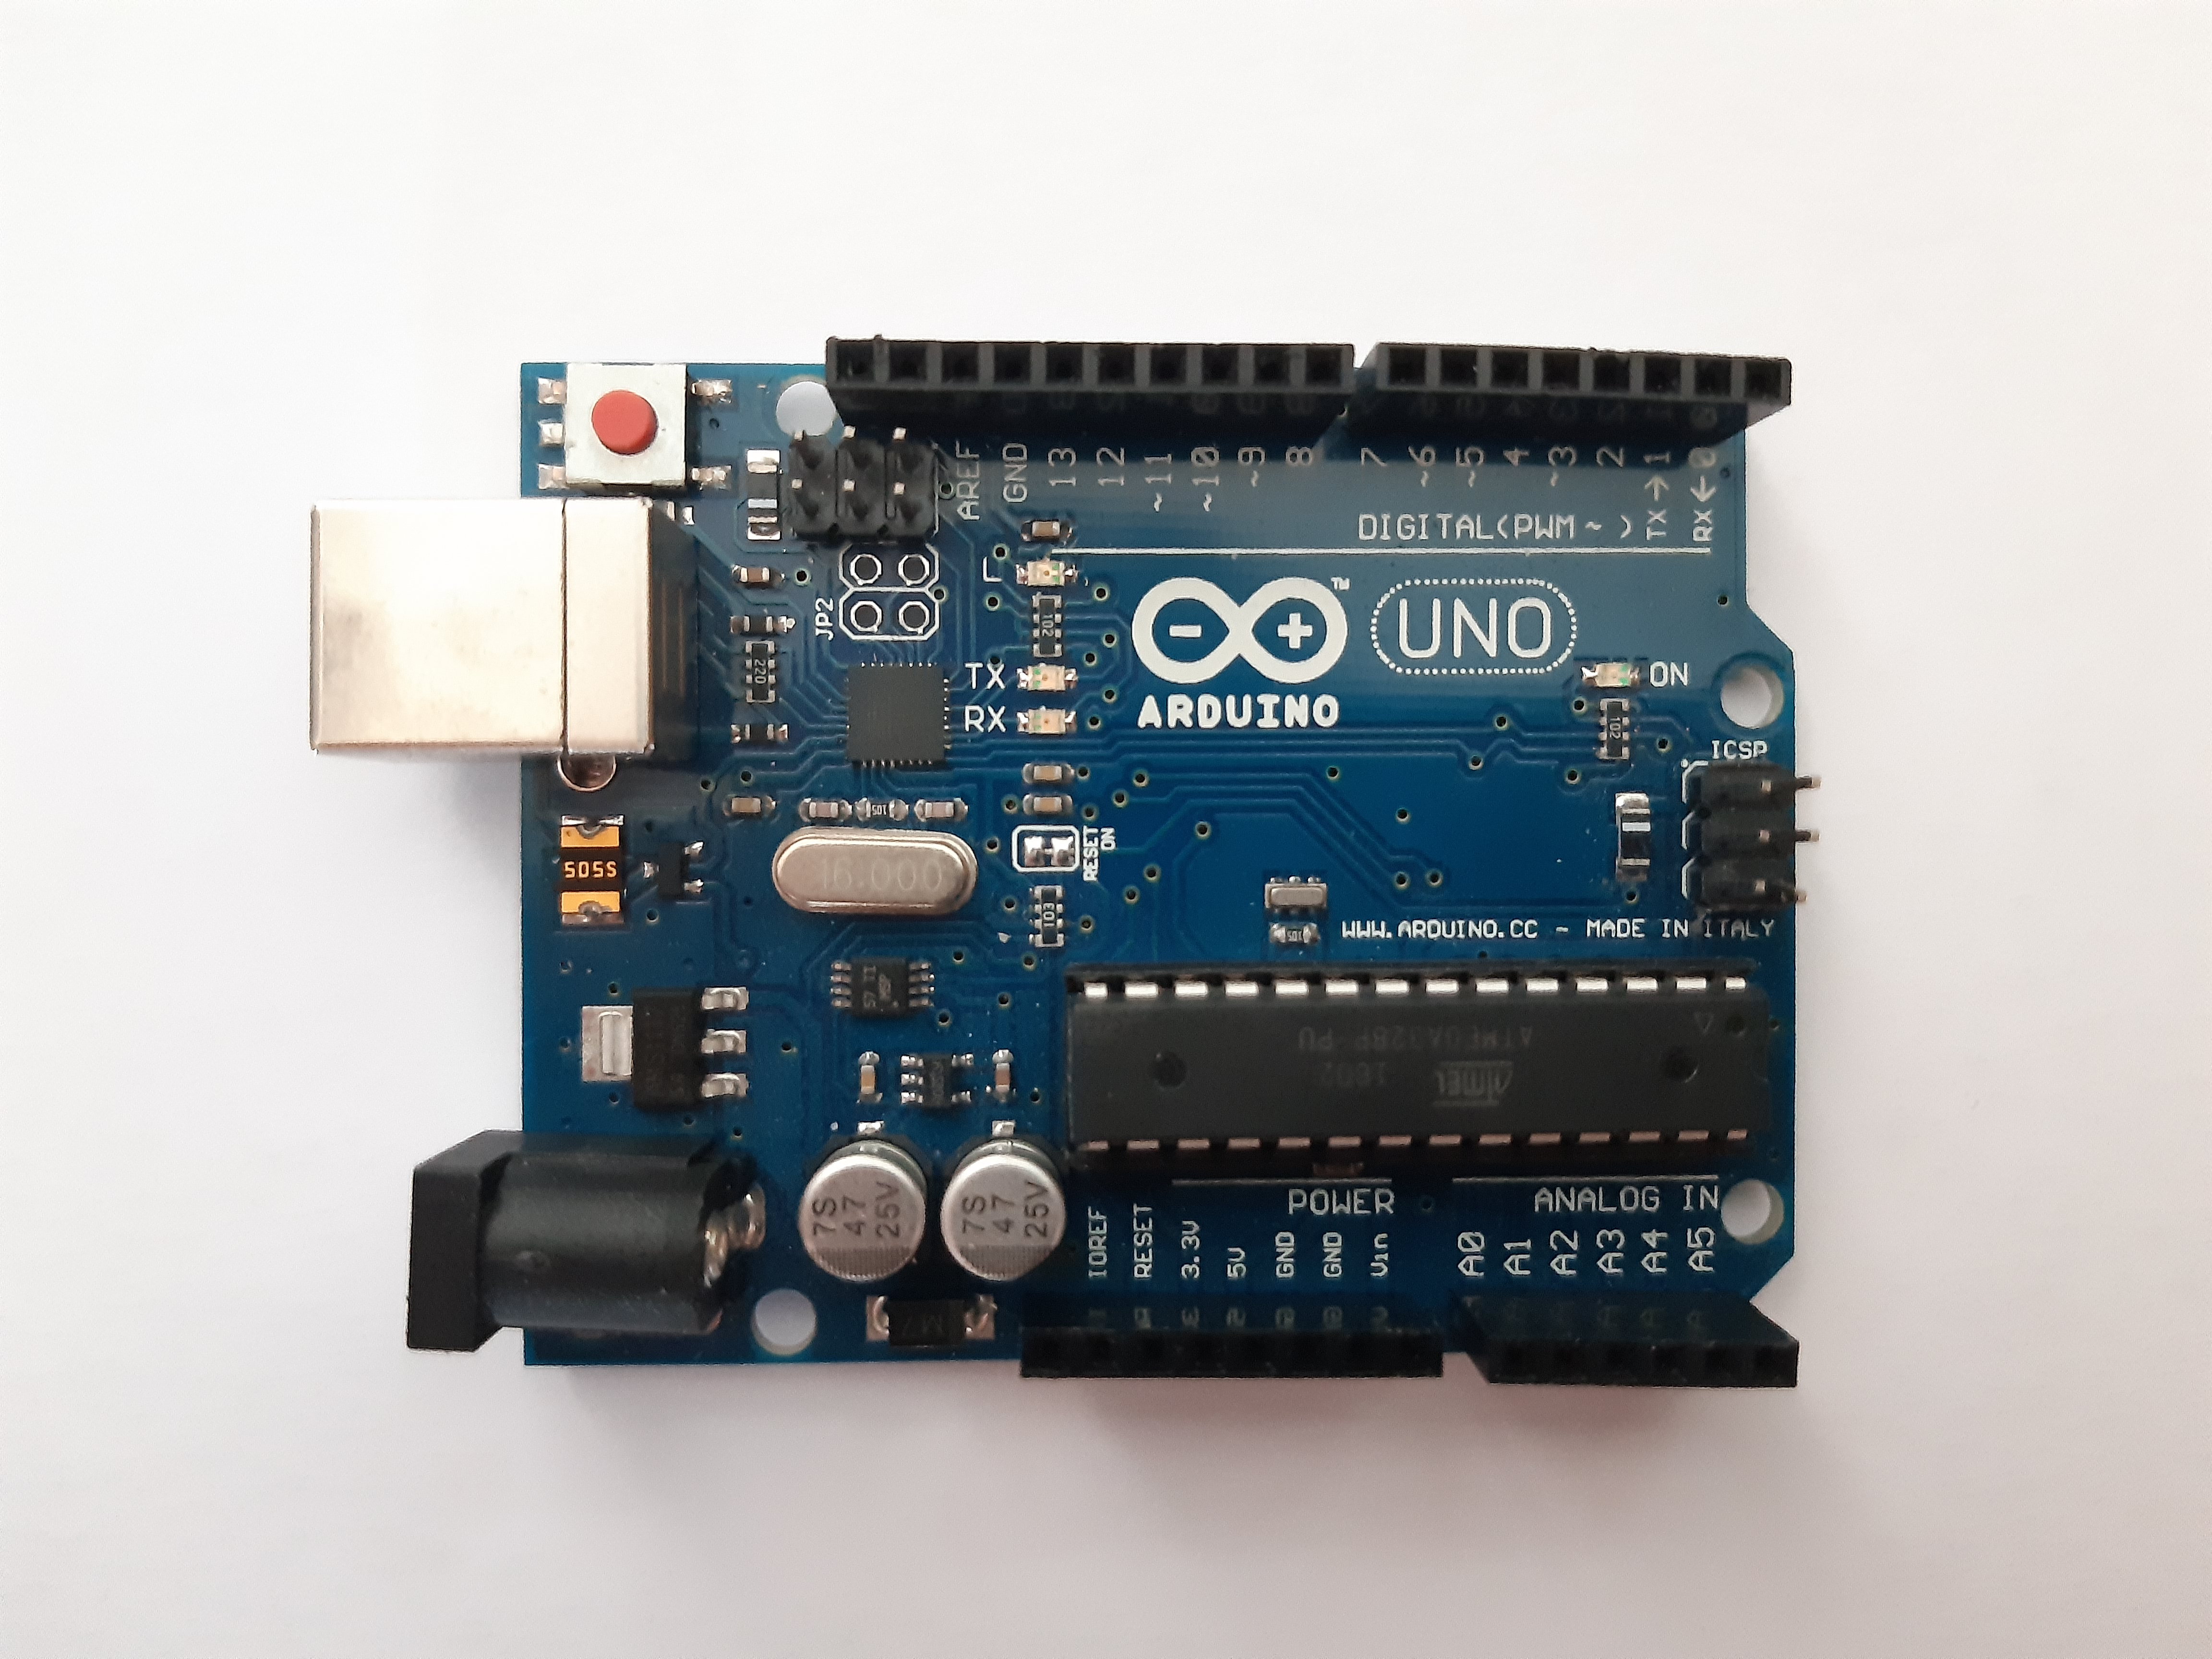
\includegraphics[width=0.5\textwidth]{img/imgArduinoUNO.jpg}
    \caption{Placa de Arduino UNO.}
    \label{fig:arduino} % Esta etiqueta es la que permite que se encuentr referenciada en el texto (es muy importante que siempre estén referenciadas en el texto)
\end{figure}

\item \textbf{ProtoBoard}: placa sobre la que se construyen los circuitos electrónicos, se trata de una matriz de clavijas donde se insertan los componentes electrónicos.\ref{fig:protoboard}
% Imagen de la protoboard.
\begin{figure}[h!]
    \centering
    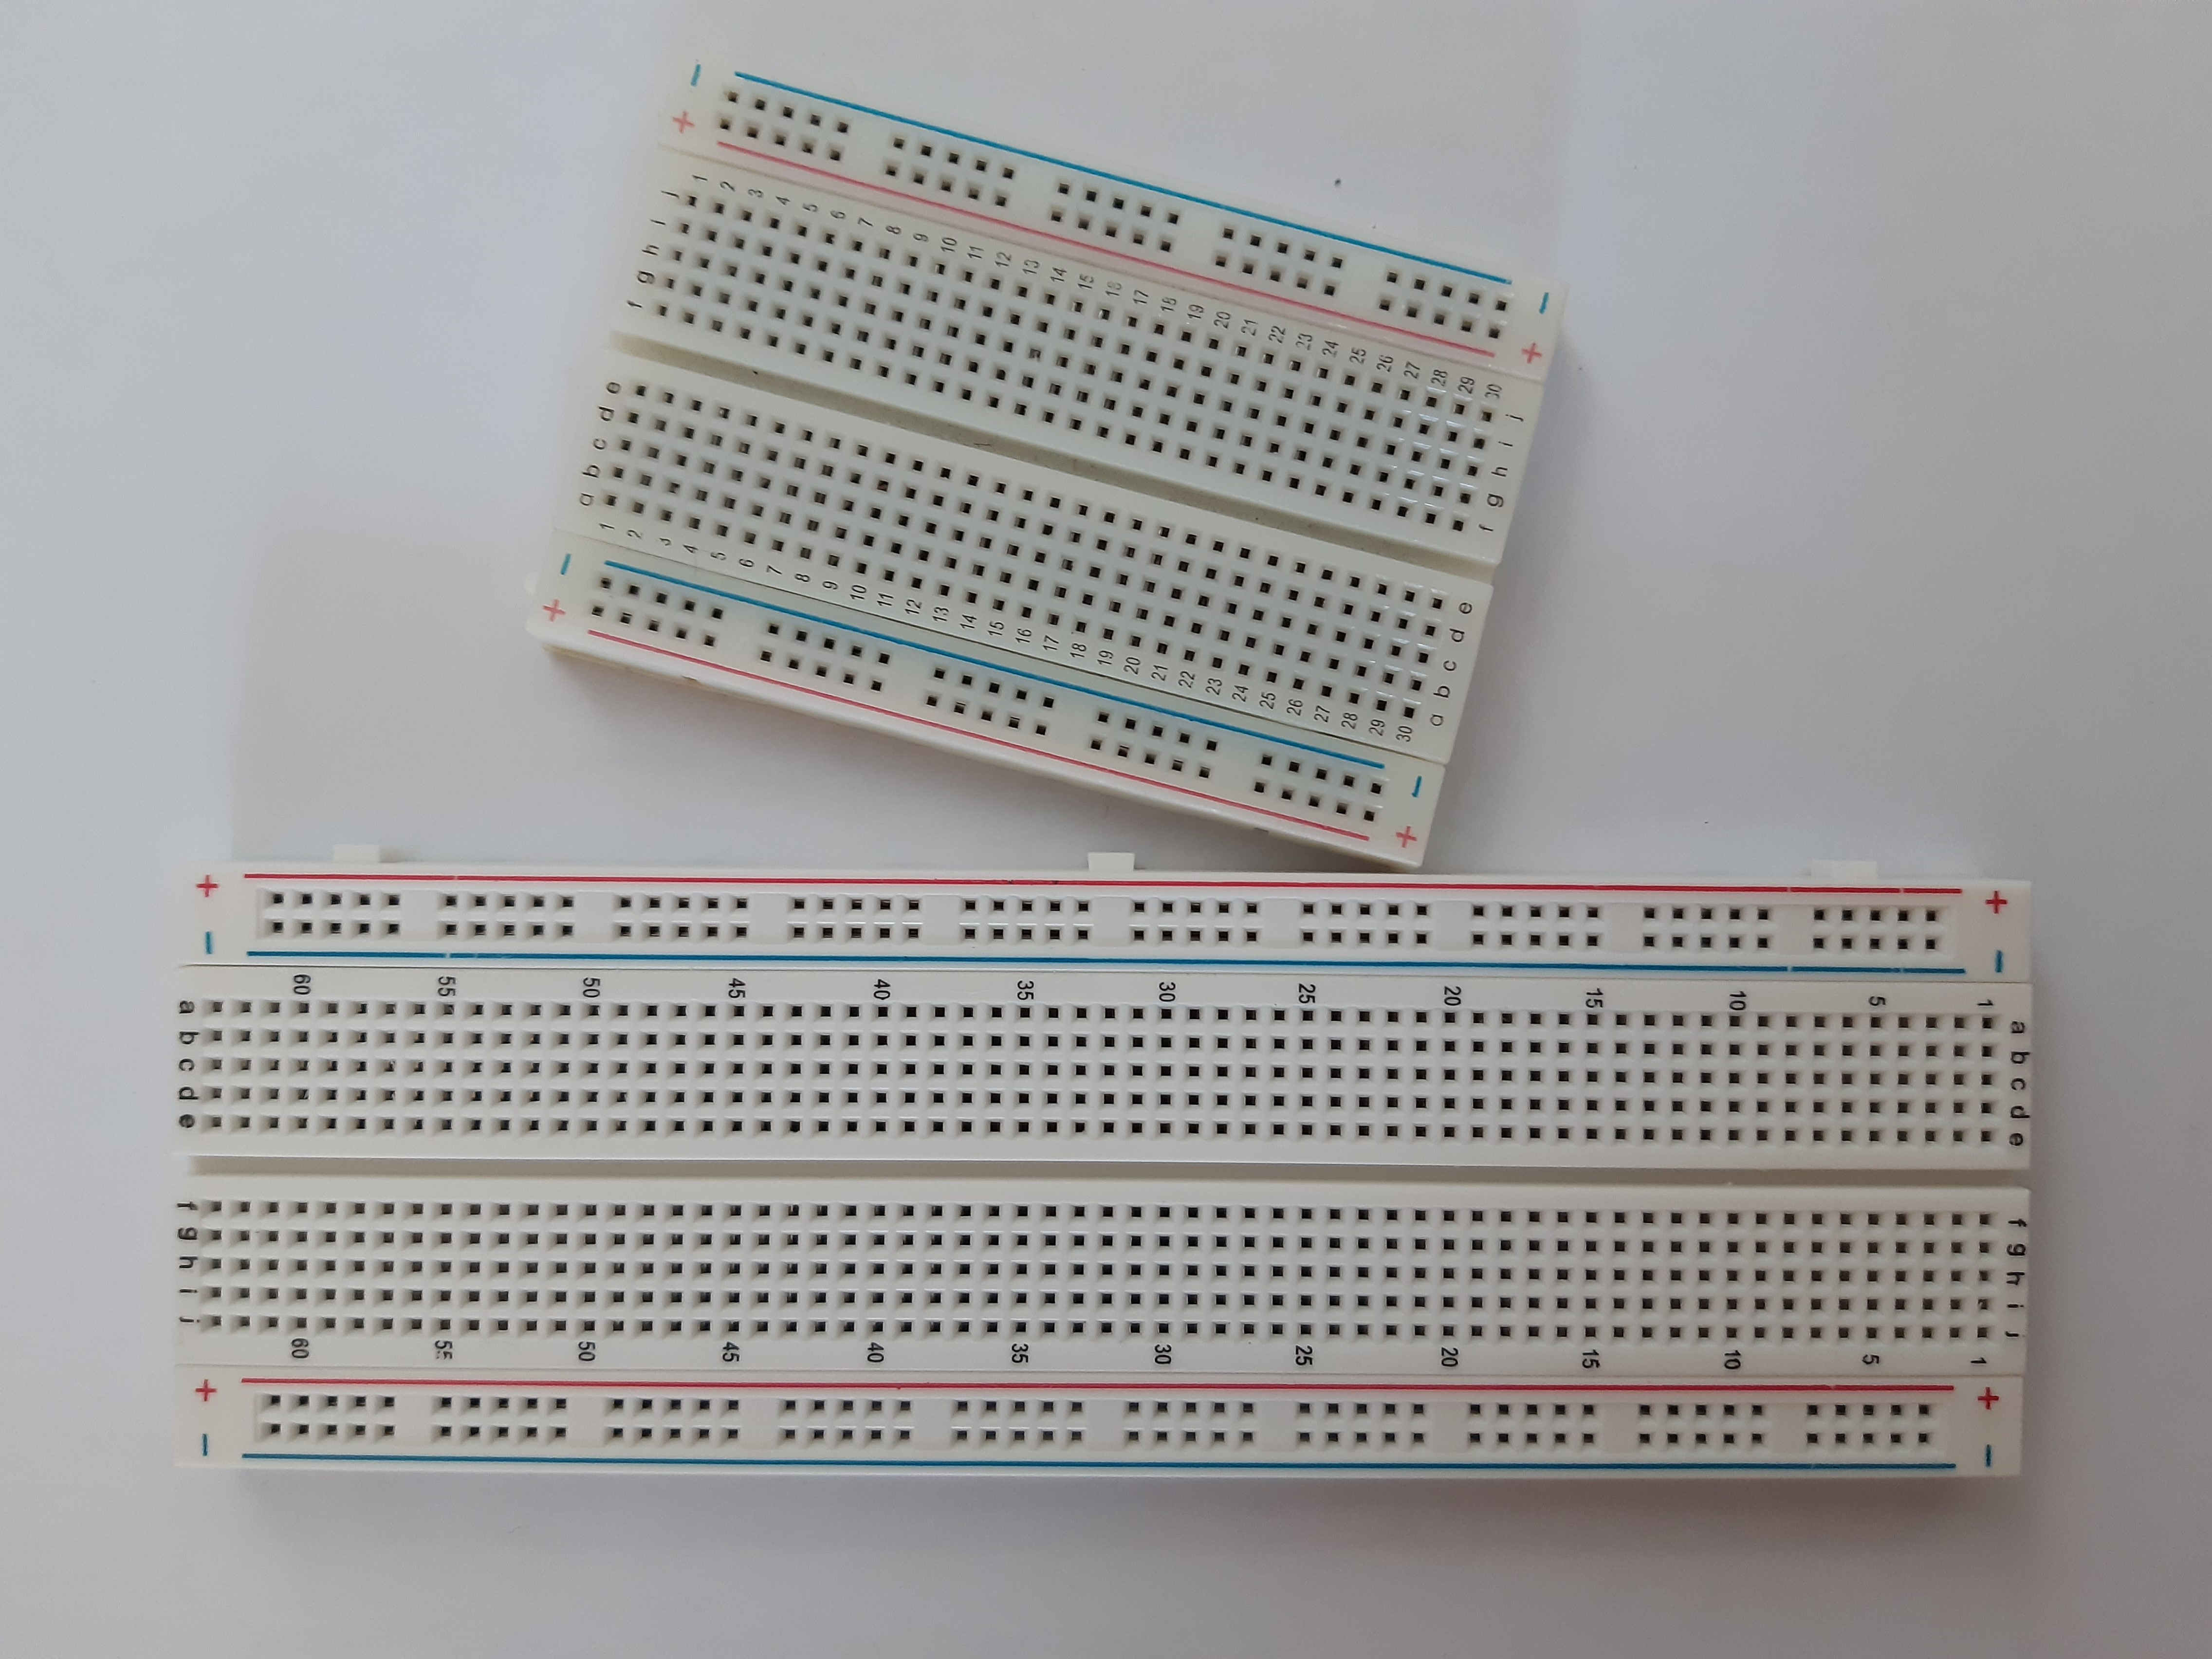
\includegraphics[width=0.5\textwidth]{img/imgProtoboards.jpg}
    \caption{Protoboards.}
    \label{fig:protoboard} % Esta etiqueta es la que permite que se encuentr referenciada en el texto (es muy importante que siempre estén referenciadas en el texto)
\end{figure}

\item \textbf{Cableado}: alambres de un material conductor cubiertos por un material aislante que permiten las distintas conexiones del circuito.\ref{fig:cableado}
% Imagen del los cables que se usarán
\begin{figure}[h!]
    \centering
    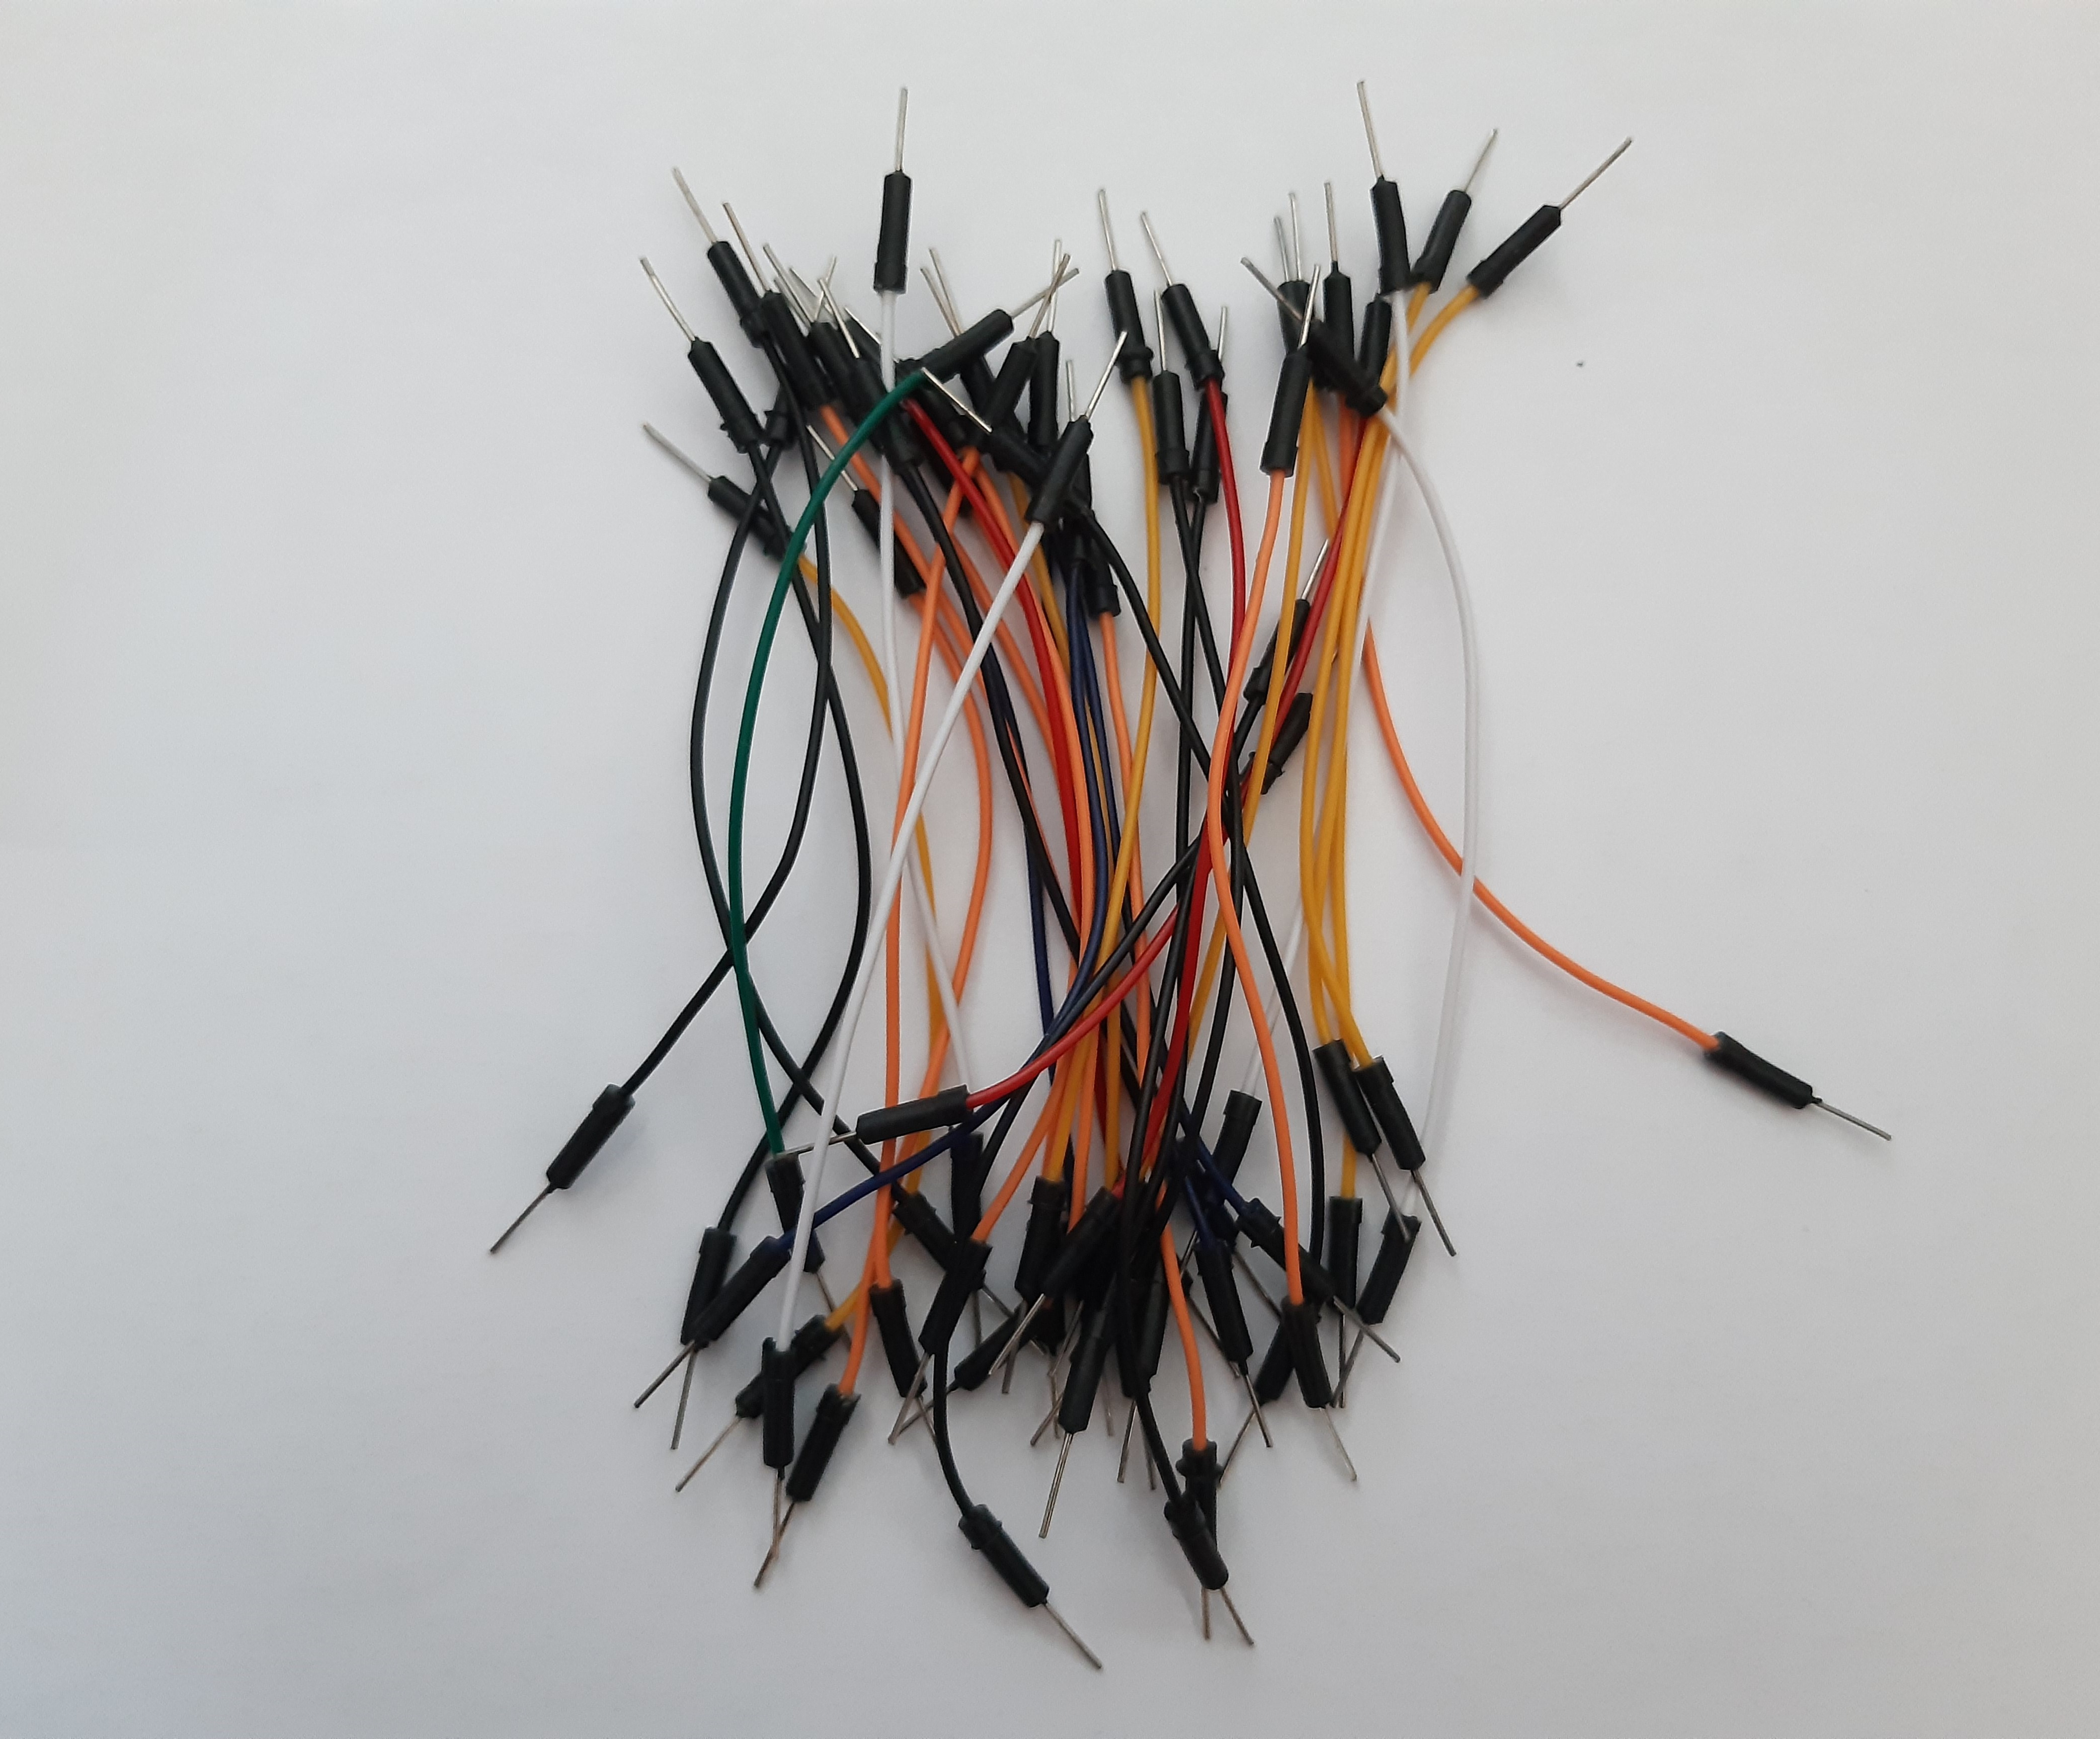
\includegraphics[width=0.4\textwidth]{img/imgCableado.jpg}
    \caption{Cables de conexiones para arduino.}
    \label{fig:cableado} % Esta etiqueta es la que permite que se encuentr referenciada en el texto (es muy importante que siempre estén referenciadas en el texto)
\end{figure}

\item \textbf{Resistencias}: componentes electrónicos que limitan el flujo de energía eléctrica del circuito. El valor de cada resistencia viene dado por un código de colores.\ref{fig:resistencias}
% Imagen de las resistencias.
\begin{figure}[h!]
    \centering
    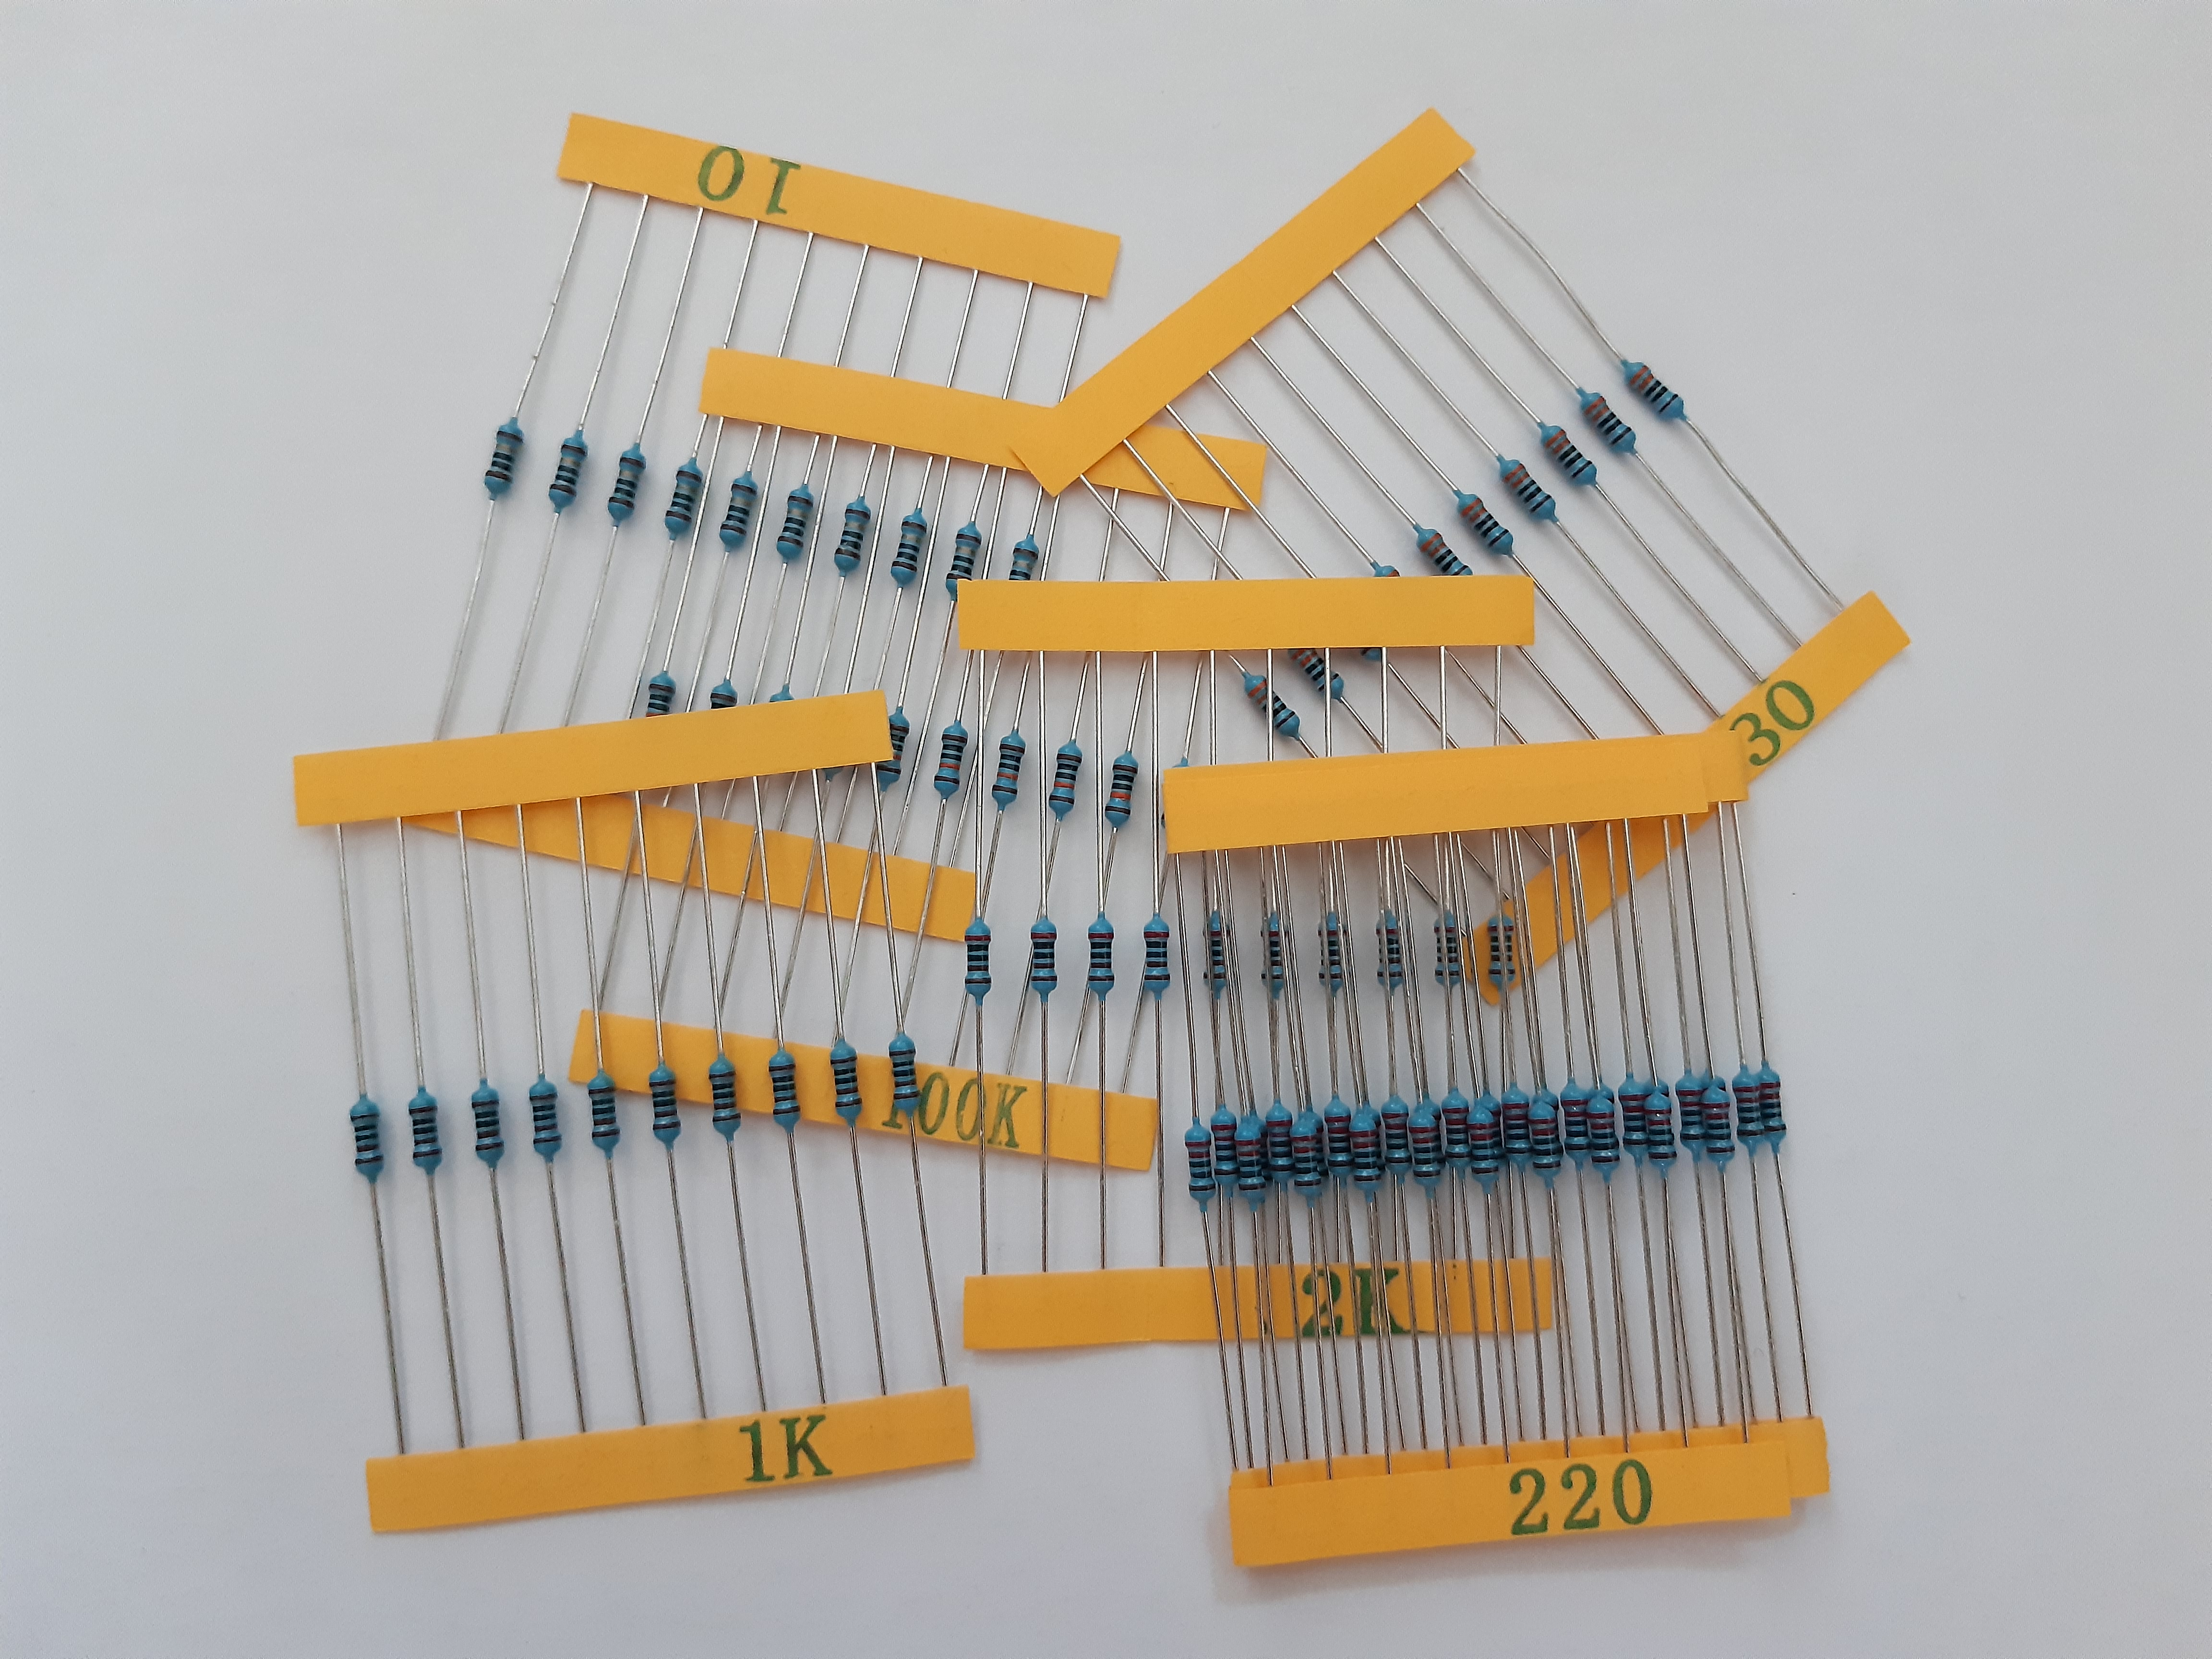
\includegraphics[width=0.5\textwidth]{img/imgResistencias.jpg}
    \caption{Distintas resistencias.}
    \label{fig:resistencias} % Esta etiqueta es la que permite que se encuentr referenciada en el texto (es muy importante que siempre estén referenciadas en el texto)
\end{figure}

\item \textbf{Leds}: diodo que se ilumina cuando pasa una corriente eléctrica por él. Existen leds de diferentes colores.\ref{fig:leds}
% imagen de los leds
\begin{figure}[h!]
    \centering
    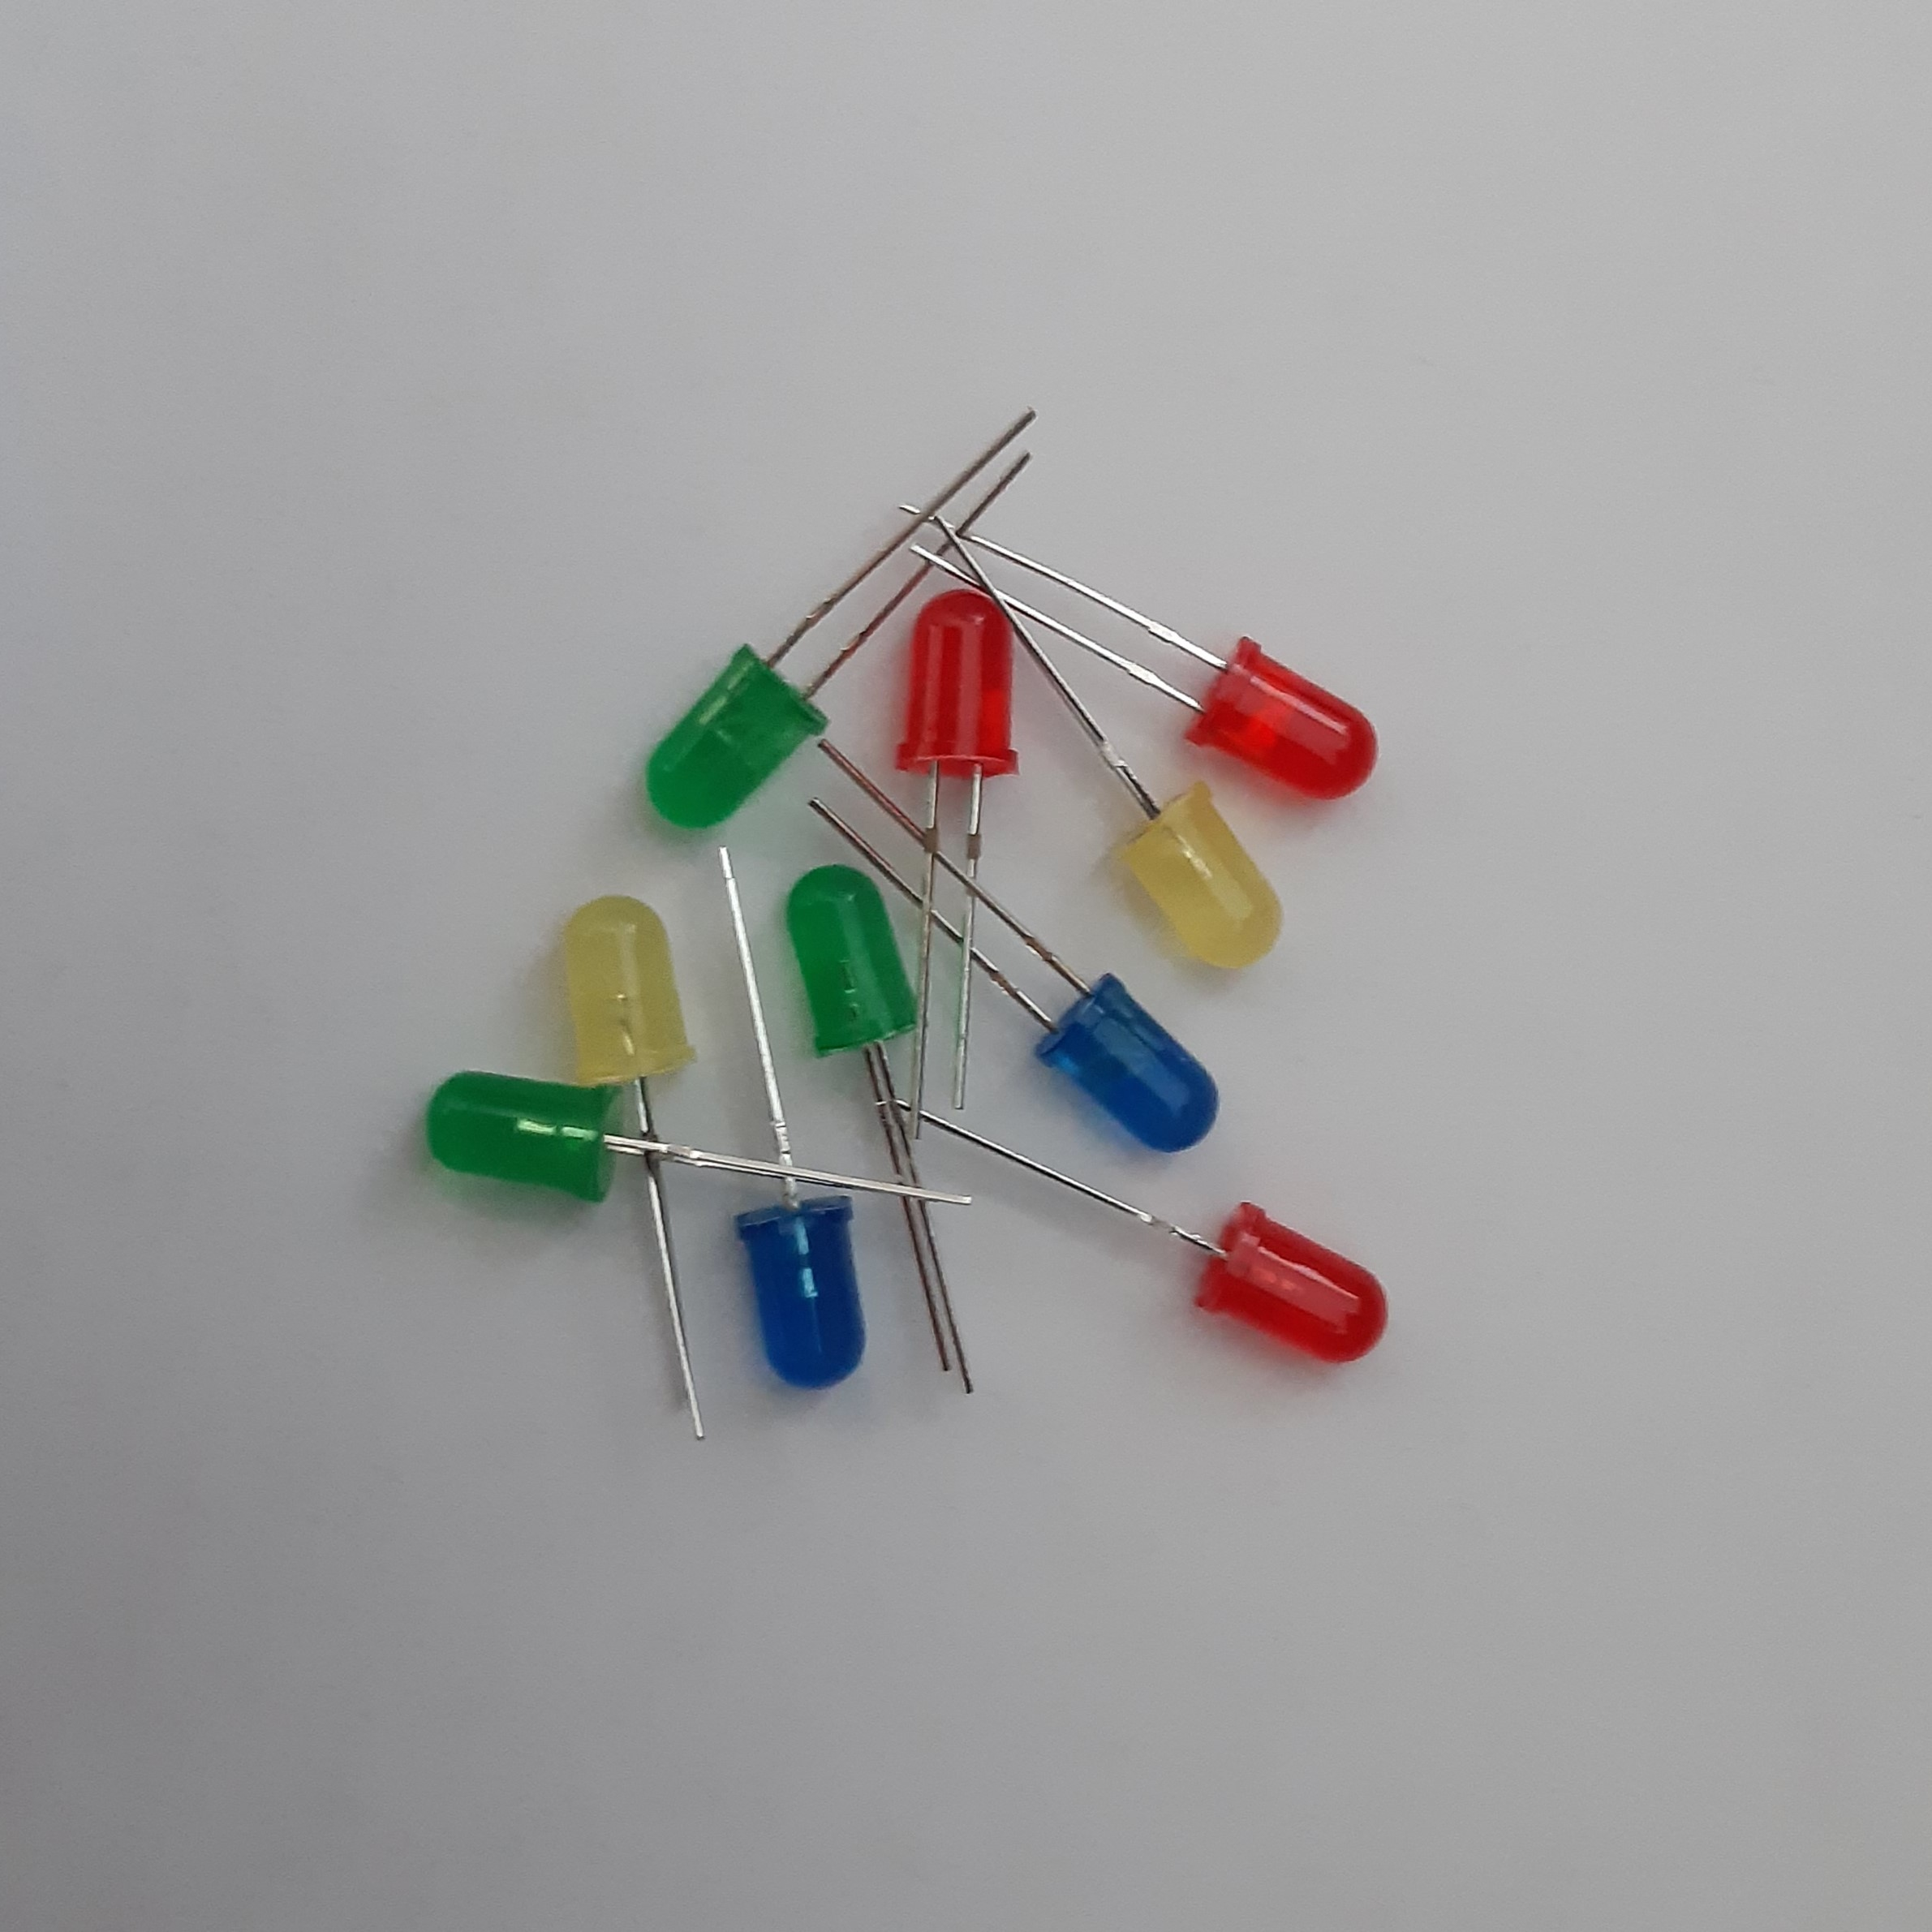
\includegraphics[width=0.4\textwidth]{img/imgLeds.jpg}
    \caption{Leds de diferentes colores.}
    \label{fig:leds} % Esta etiqueta es la que permite que se encuentr referenciada en el texto (es muy importante que siempre estén referenciadas en el texto)
\end{figure}

\item \textbf{Pulsador}: componente que según su estado permite cortar o admitir el paso de corriente. En función de su estado se realizará una acción específica u otra.\ref{fig:pulsador}
% Imagen de pulsadores de arduino
\begin{figure}[h!]
    \centering
    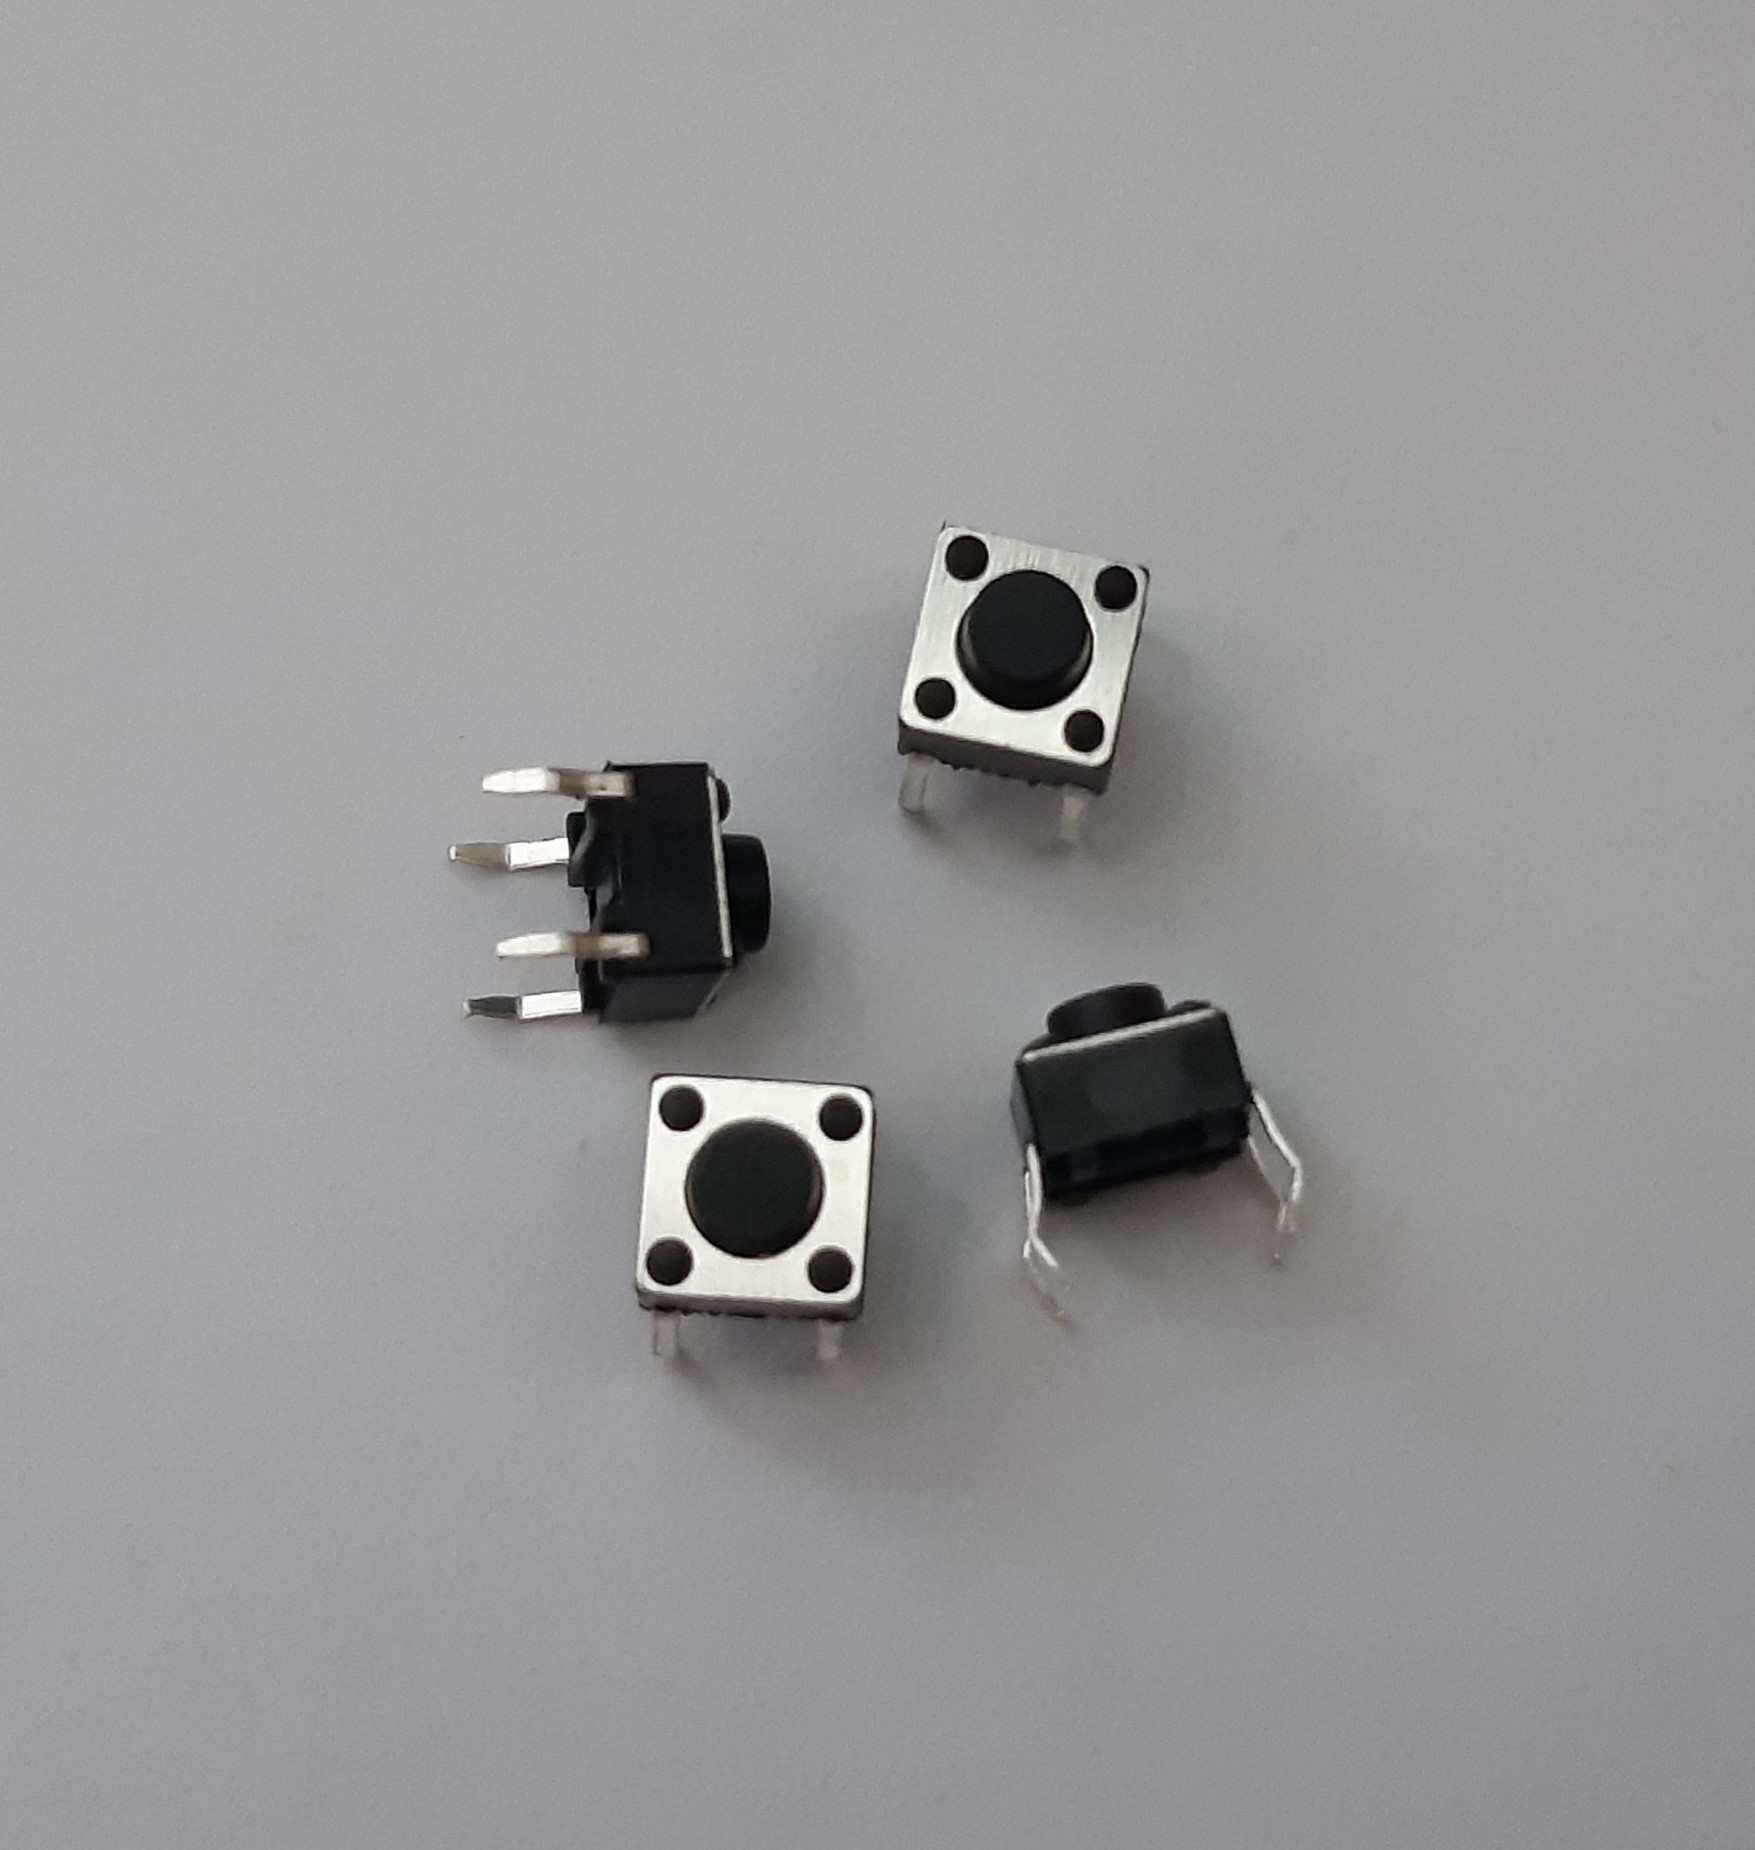
\includegraphics[width=0.4\textwidth]{img/imgPulsador.jpg}
    \caption{Pulsadores.}
    \label{fig:pulsador} % Esta etiqueta es la que permite que se encuentr referenciada en el texto (es muy importante que siempre estén referenciadas en el texto)
\end{figure}

\item \textbf{Cable USB}: conector que permite introducir las instrucciones programadas en un ordenador a la placa de Arduino.\ref{fig:cableUSB}
% Imagen del cable USB que conecta el arduino
\begin{figure}[h!]
    \centering
    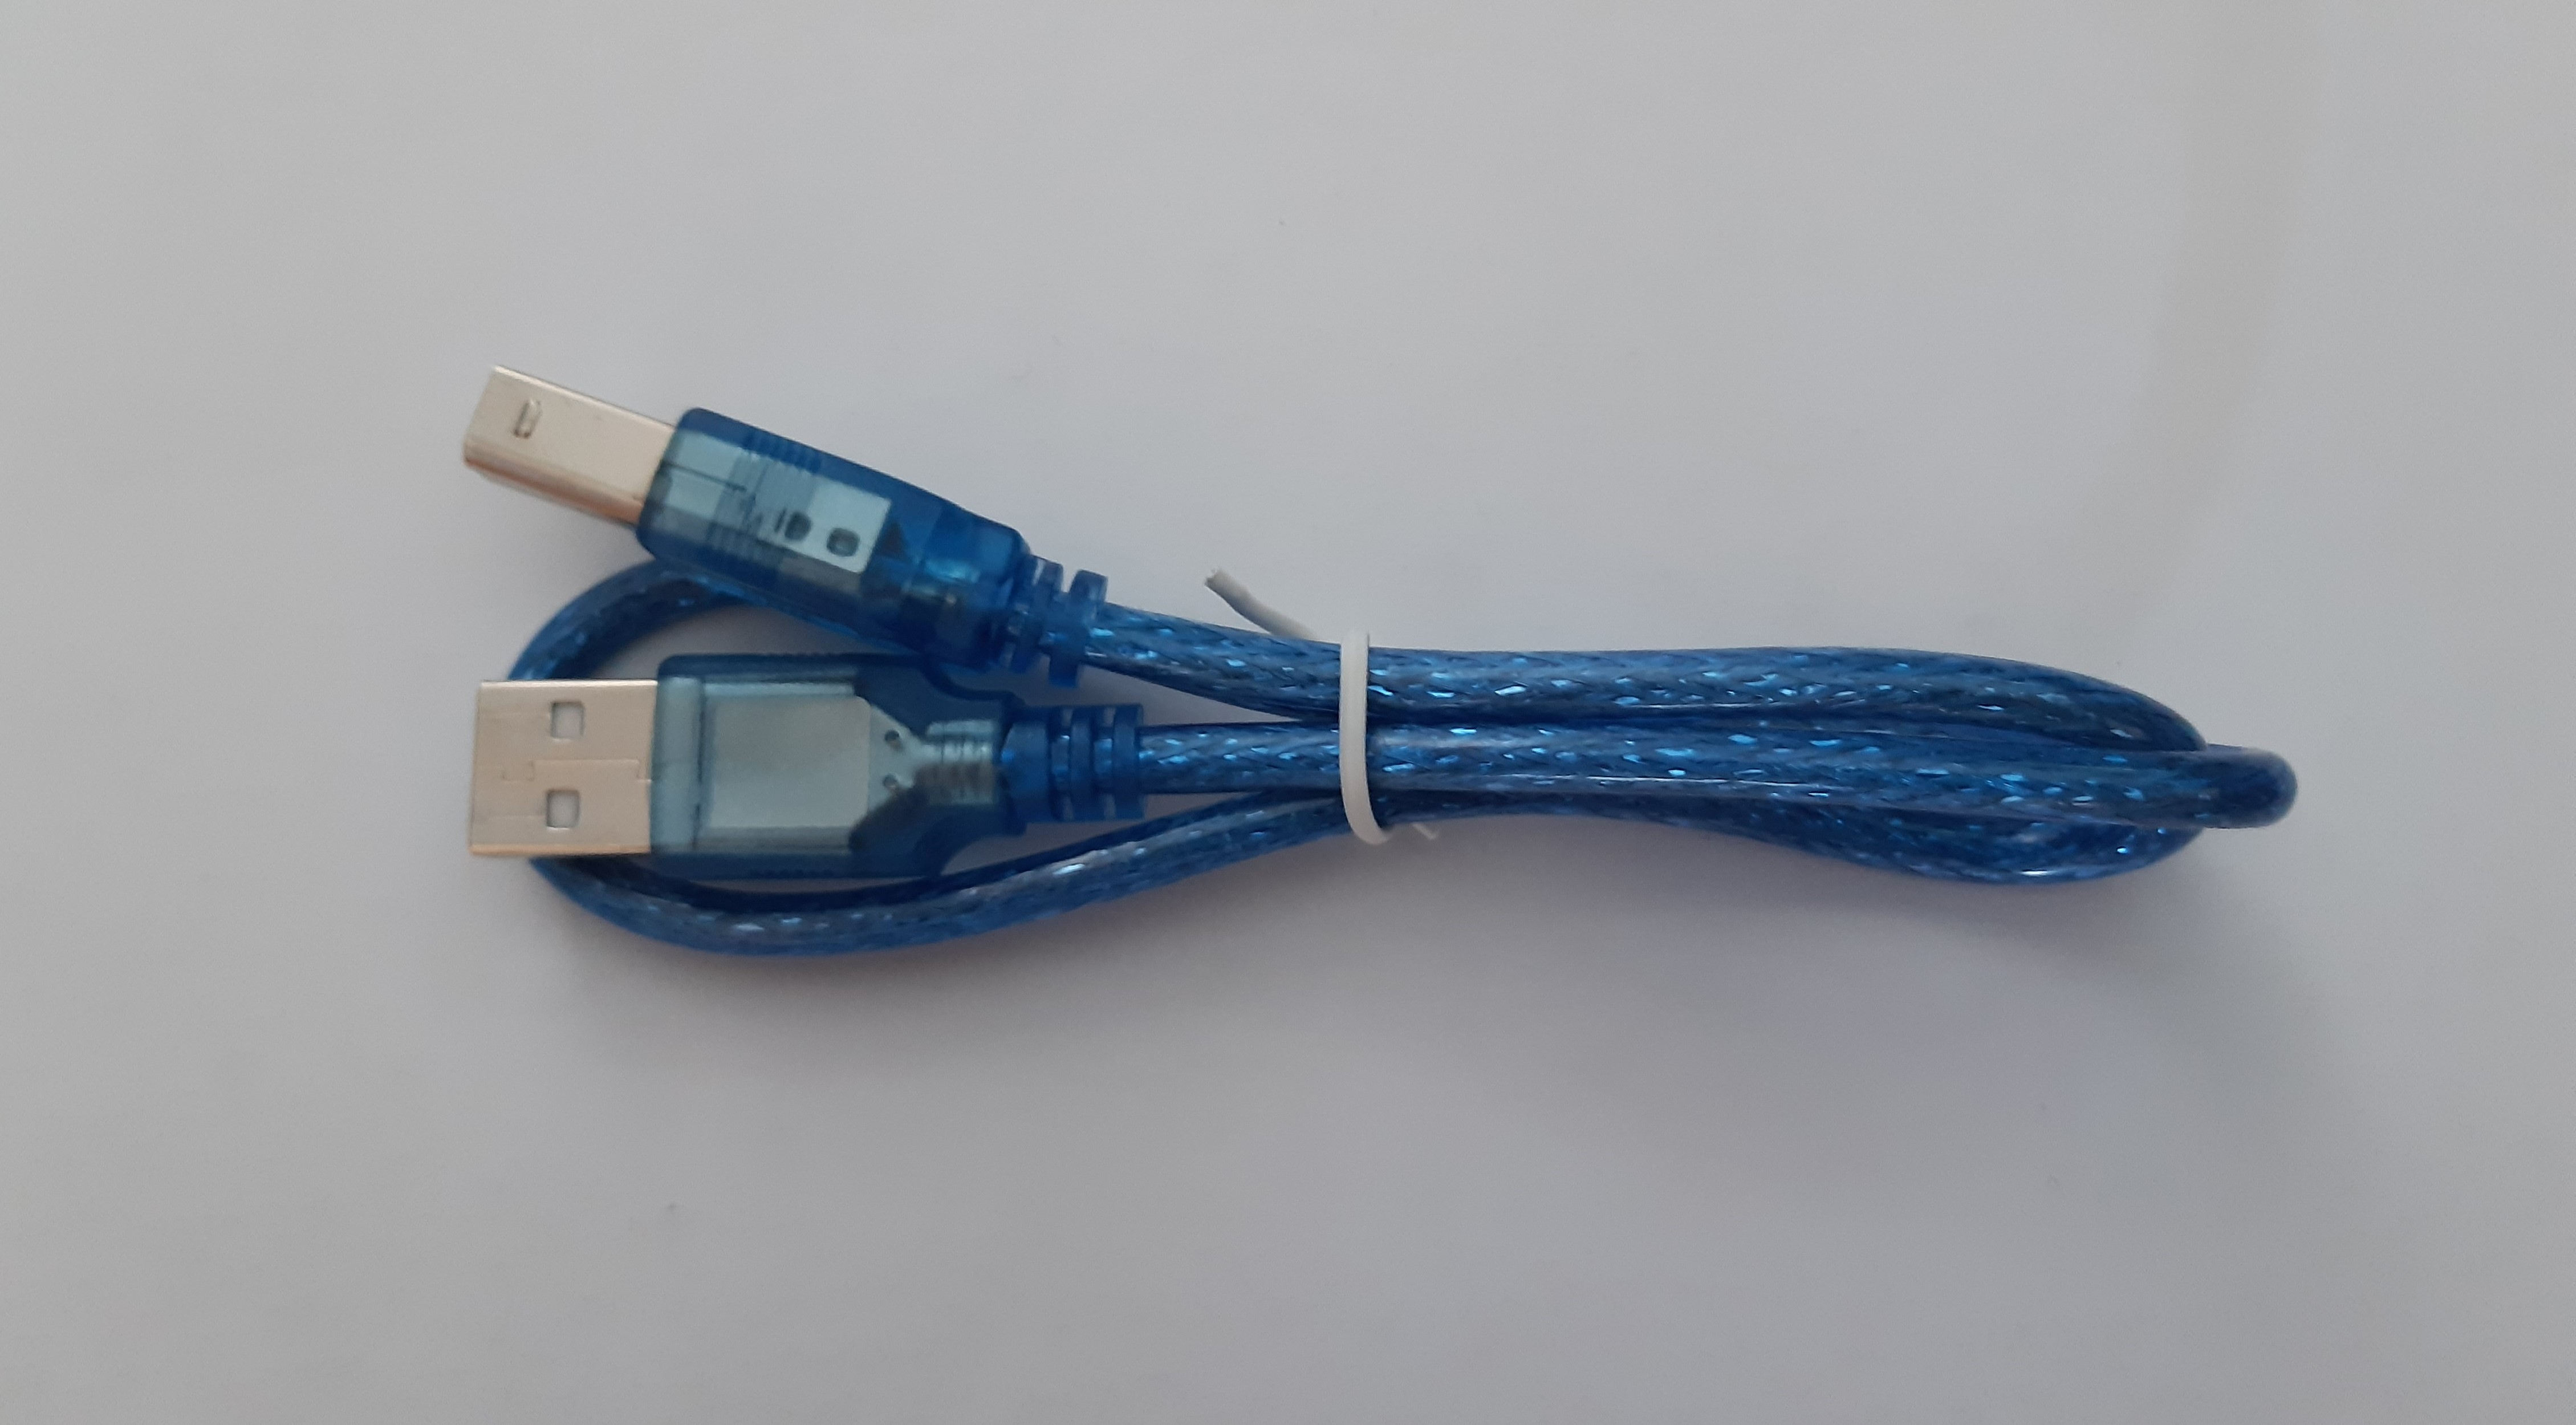
\includegraphics[width=0.5\textwidth]{img/imgCableUSB.jpg}
    \caption{Cable USB.}
    \label{fig:cableUSB} % Esta etiqueta es la que permite que se encuentr referenciada en el texto (es muy importante que siempre estén referenciadas en el texto)
\end{figure}

\item \textbf{Motor de vibración}: componente electrónico que al alimentarlo causa un efecto vibratorio. En este proyecto su finalidad será la de alertar al usuario mediante un biofeedback de señal vibratoria.\ref{fig:motorVibr}
% Imagen de un motor de vibración
\begin{figure}[h!]
    \centering
    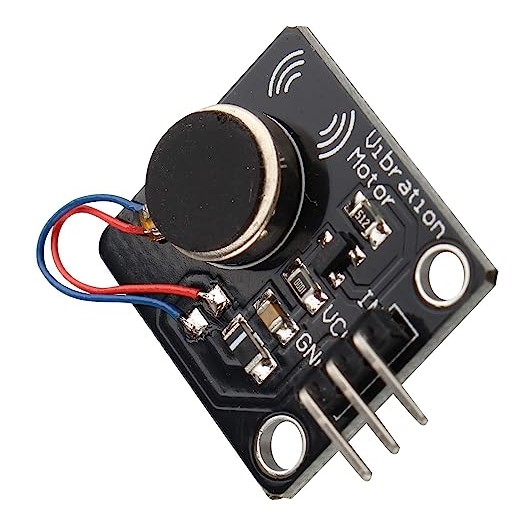
\includegraphics[width=0.5\textwidth]{img/MotorVibr.jpg}
    \caption{Motor de vibración.\cite{imgMotorVibr}}
    \label{fig:motorVibr} % Esta etiqueta es la que permite que se encuentr referenciada en el texto (es muy importante que siempre estén referenciadas en el texto)
\end{figure}

\item \textbf{Zumbador pasivo}: un transductor electroacústico que transforma una señal acústica en un efecto sonoro. En este proyecto su finalidad será la de alertar al usuario mediante un biofeedback de señal sonora.\ref{fig:zumbador}
% Imagen de un zumbador pasivo.
\begin{figure}[h!]
    \centering
    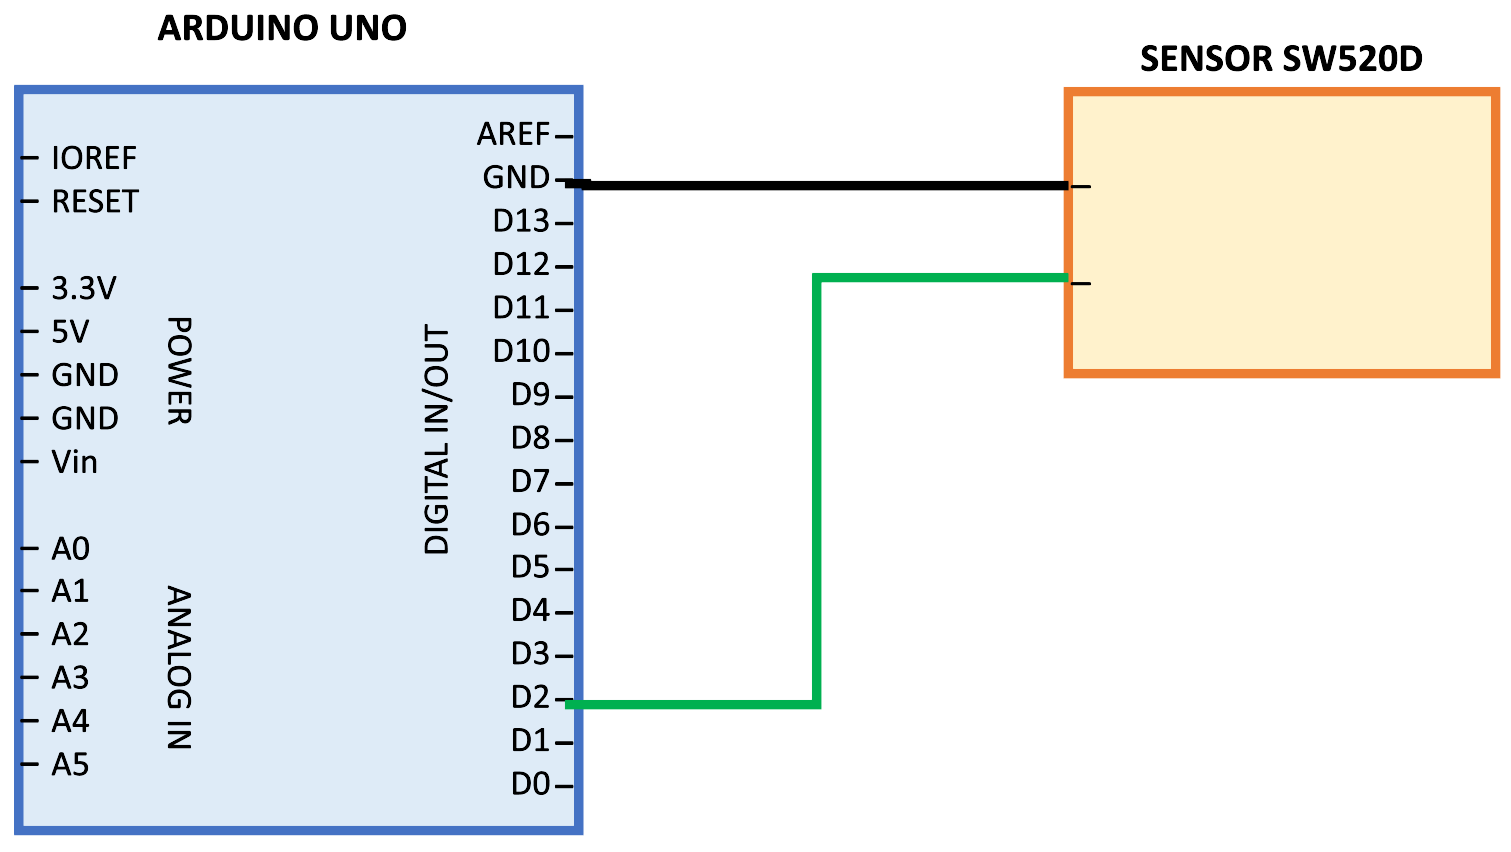
\includegraphics[width=0.5\textwidth]{img/SW520D.png}
    \caption{Zumbador pasivo.}
    \label{fig:zumbador} % Esta etiqueta es la que permite que se encuentr referenciada en el texto (es muy importante que siempre estén referenciadas en el texto)
\end{figure}

\end{itemize}


\subsubsection{Posibles sensores.}

\begin{itemize}
    \item \textbf{Módulo SCA60C}\cite{SCA60C}: módulo que consta de un sensor de ángulo SCA60C y un acelerómetro N100060. Gracias a este sensor se pueden medir ángulos de 0 a 180º, con resolución de un grado, con un voltaje de entrada de 5 voltios y una tensión de salida en función del ángulo de 0,45 - 4,5 voltios. La corriente que necesita módulo ronda los 2 mA. Este módulo admite distintos rangos de medición y se utiliza para multitud de aplicaciones en las que se necesite conocer constantemente el ángulo de giro. 
% Imagen Módulo SCA60C
\begin{figure}[h!]
    \centering
    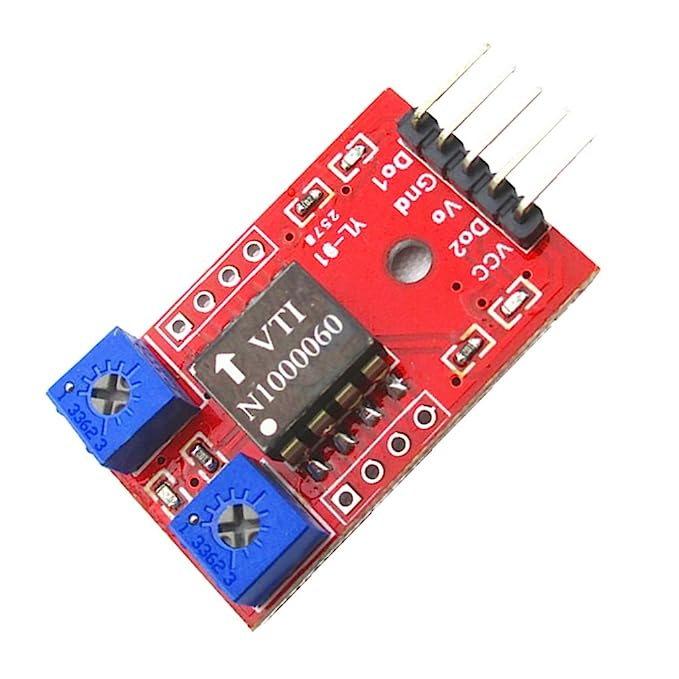
\includegraphics[width=0.3\textwidth]{img/imgSCA60C.jpg}
    \caption{Módulo SCA60C\cite{imgSCA60C}.}
    \label{fig:SCA60C} % Esta etiqueta es la que permite que se encuentr referenciada en el texto (es muy importante que siempre estén referenciadas en el texto)
\end{figure}

    
    \item \textbf{Galgas extensiométricas y módulo HX711}\cite{GyHX711_1,GyHX711_2}: se trata de un conjunto cuyo objetivo es medir el peso, basado en un transductor de galgas extensiométricas y un módulo HX711 que actúa como amplificador de la señal y transfiere los datos al microcontrolador. La galga extensiométrica o celda de carga es un transductor que convierte la tensión generada por los cambios en la longitud de un objeto a una señal eléctrica, en función del peso que se quiere medir existen distintas celdas de carga. Mientras que el módulo HX711 consta de un amplificador y un convertidor analógico-digital HX711, que permite la amplificación de la señal producida por la galga extensiométrica. Este módulo utiliza un puente de Weahstone para convertir la fuerza aplicada en una señal analógica. Necesita una tensión de entrada de 5 voltios y el resultado se puede obtener en g, kg o Newtons. La utilización de este módulo requiere de la librería de Arduino hx711. El precio ronda los 10-15€.
% Imagen de galgas extensiometricas y el módulo HX711
\begin{figure}[h!]
    \centering
    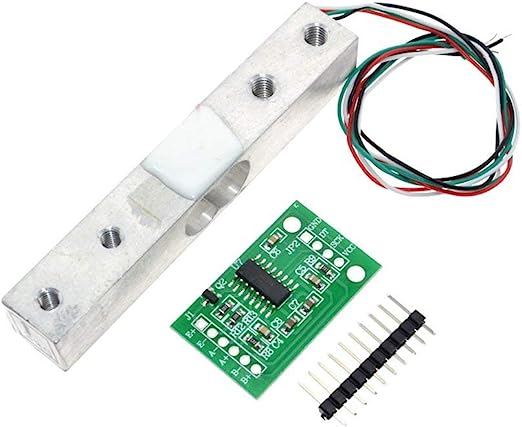
\includegraphics[width=0.3\textwidth]{img/GyHX711.jpg}
    \caption{Galgas extensiométricas y módulo HX711\cite{imgGyHX711}.}
    \label{fig:HX711} % Esta etiqueta es la que permite que se encuentr referenciada en el texto (es muy importante que siempre estén referenciadas en el texto)
\end{figure}

    \item \textbf{Acelerómetro ADXL345}\cite{ADXL345}: acelerómetro micromecanizado (MEMS) capacitivo de 3 grados de Libertad (3DOF\footnote{\textbf{DOF: Degrees of Freedom, los grados de libertad, hace referencia a la cantidad de ejes en los que un sensor puede realizar su medición}}) acoplado a un bloque de memoria FIFO que almacena hasta 32 conjuntos de coordenadas. Además, es compatible con un procesador como Arduino mediante conexión por bus SPI o bus I2C. Este dispositivo permite conocer la orientación del sensor por la acción de la fuerza de gravedad basándose en la detección de la aceleración en los ejes X, Y y Z. Se trata de un dispositivo de ultra bajo consumo, únicamente consume en funcionamiento unos 45 $\mu$A de corriente mientras que en Stand-By solamente consume unos 0,1 $\mu$A. Este acelerómetro necesita una tensión de alimentación de unos 2 a 3,6 voltios. El rango de medición del dispositivo es ajustable, con resolución de hasta 13 bits y sensibilidad de 40 mg/LBS.
% Imagen del acelerómetro ADXL345
\begin{figure}[h!]
    \centering
    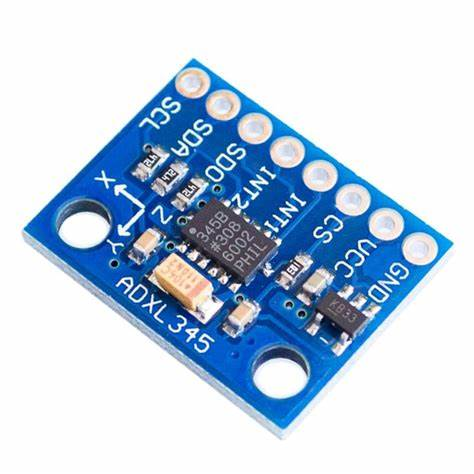
\includegraphics[width=0.2\textwidth]{img/ADXL345.jpeg}
    \caption{Acelerómetro ADXL345\cite{imgADXL345}.}
    \label{fig:ADXL345} % Esta etiqueta es la que permite que se encuentr referenciada en el texto (es muy importante que siempre estén referenciadas en el texto)
\end{figure}

    \item \textbf{Módulo SW520D}\cite{SW520D_1}: Sensor de inclinacion formado por sensores Tilt de doble esfera. Este sensor funciona como un intrerruptor y tiene una salida digital, al inclinar el sensor las 2 esferas actúan de puente y cierran el circuito. El código de programación de este dispositivo es similar al de un interruptor. Se trata de un sensor muy sensible a movimientos bruscos y vibraciones. Sin embargo, es un sensor muy barato.
    % Referencia: 
    % https://www.luisllamas.es/medir-inclinacion-con-arduino-y-sensor-tilt-sw-520d/
% Imagen del sensor SW520D
\begin{figure}[h!]
    \centering
    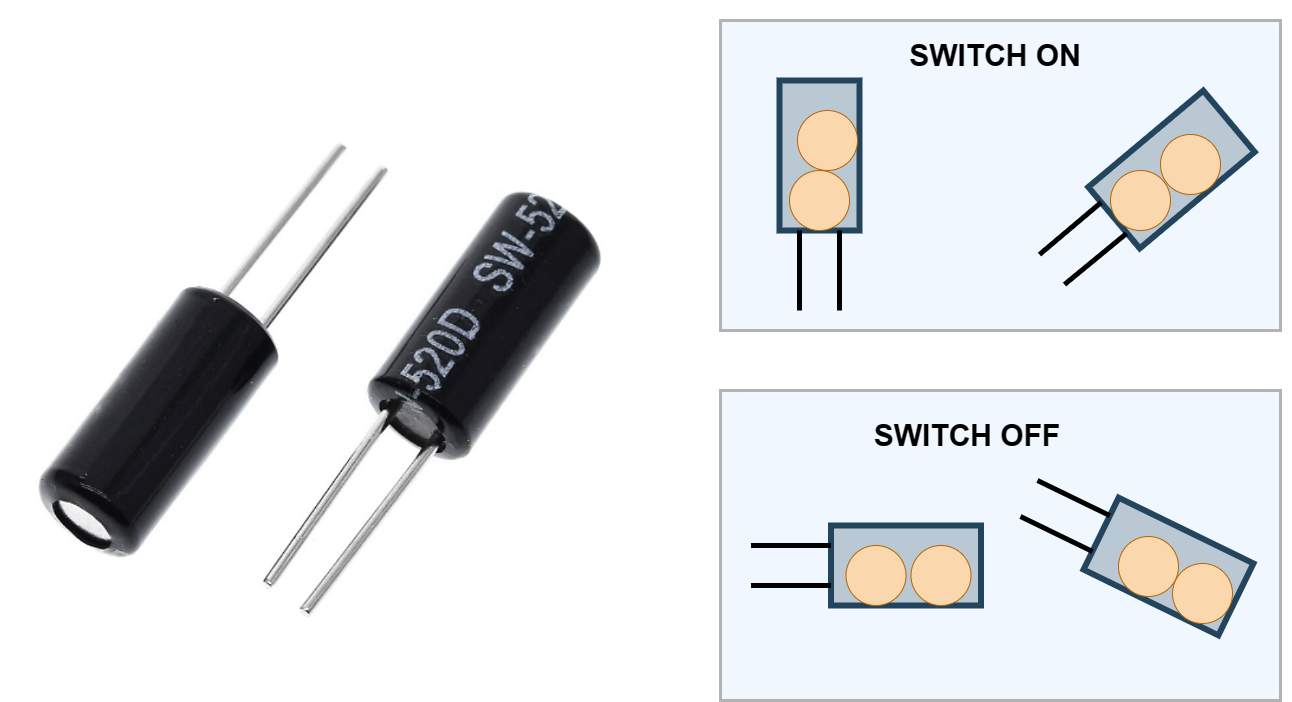
\includegraphics[width=0.4\textwidth]{img/imgSW520D_diag.png}
    \caption{Sensor SW520D\cite{imgSW520D} y diagrama de su funcionamiento.}
    \label{fig:imgSW520D} % Esta etiqueta es la que permite que se encuentr referenciada en el texto (es muy importante que siempre estén referenciadas en el texto)
\end{figure}

% Diagrama del sensor SW520D
\begin{figure}[h!]
    \centering
    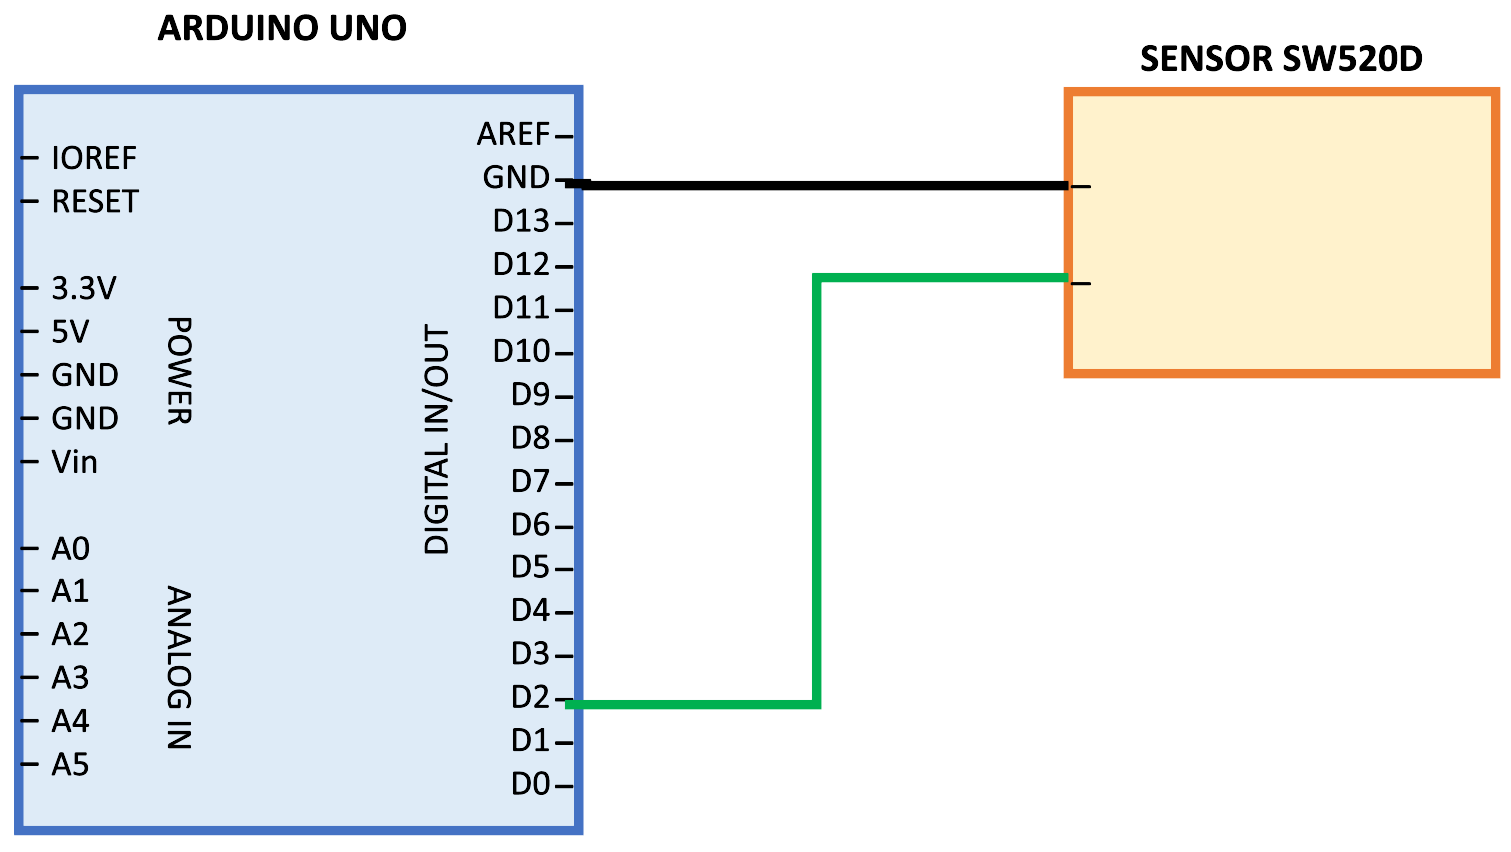
\includegraphics[width=0.5\textwidth]{img/SW520D.png}
    \caption{Diagrama de las conexiones del sensor SW520D.}
    \label{fig:SW520D} % Esta etiqueta es la que permite que se encuentr referenciada en el texto (es muy importante que siempre estén referenciadas en el texto)
\end{figure}

    \item \textbf{IMU MPU-6050}\cite{MPU6050_1,MPU6050_2}: es un módulo de unidad de medición inercial de 6 grados de libertad (6 DOF) fabricado por Invensense\textcolor{red}{referencia de la empresa}, que permite conocer la posición del sensor en todo momento. Este módulo consta de un acelerómetro de 3 ejes, un giroscopio de 3 ejes, conversores analógico a digital (ADC) de 16 bits, un sensor de temperatura, un reloj de alta precisión e interrupciones programables y un procesador interno (DMP Digital Motion Porcessor). Tanto el rango del acelerómetro como del giroscopio son ajustables. Este módulo se acopla mediante un bus SPI o un bus I2C, necesita una tensión de alimentación de unos 2,4 - 3,6 voltios, aunque hay algunos módulos que tienen incluido un regulador de voltaje que permite su conexión a un voltaje de 5V, y consume unos 3,5 mA al tener todos sus componentes activados. Es uno de los sensores más empleados y tiene un coste de unos 6-15€.
% Imagen del módulo MPU6050
\begin{figure}[h!]
    \centering
    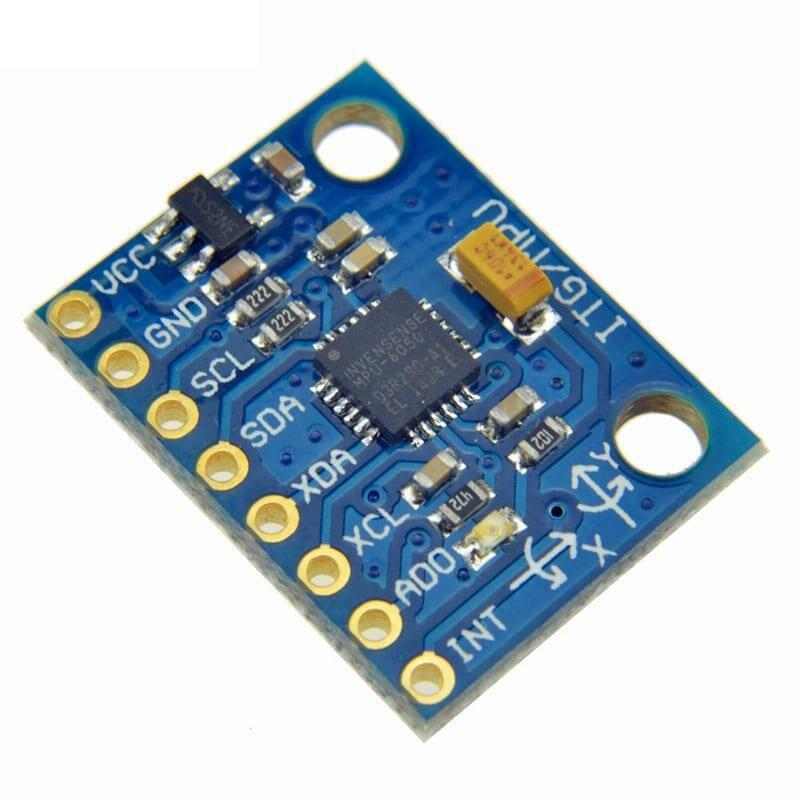
\includegraphics[width=0.2\textwidth]{img/imgMPU6050.jpg}
    \caption{Módulo MPU-6050\cite{imgMPU6050}.}
    \label{fig:imgMPU6050} % Esta etiqueta es la que permite que se encuentr referenciada en el texto (es muy importante que siempre estén referenciadas en el texto)
\end{figure}
% Diagrama del sensor MPU6050
\begin{figure}[h!]
    \centering
    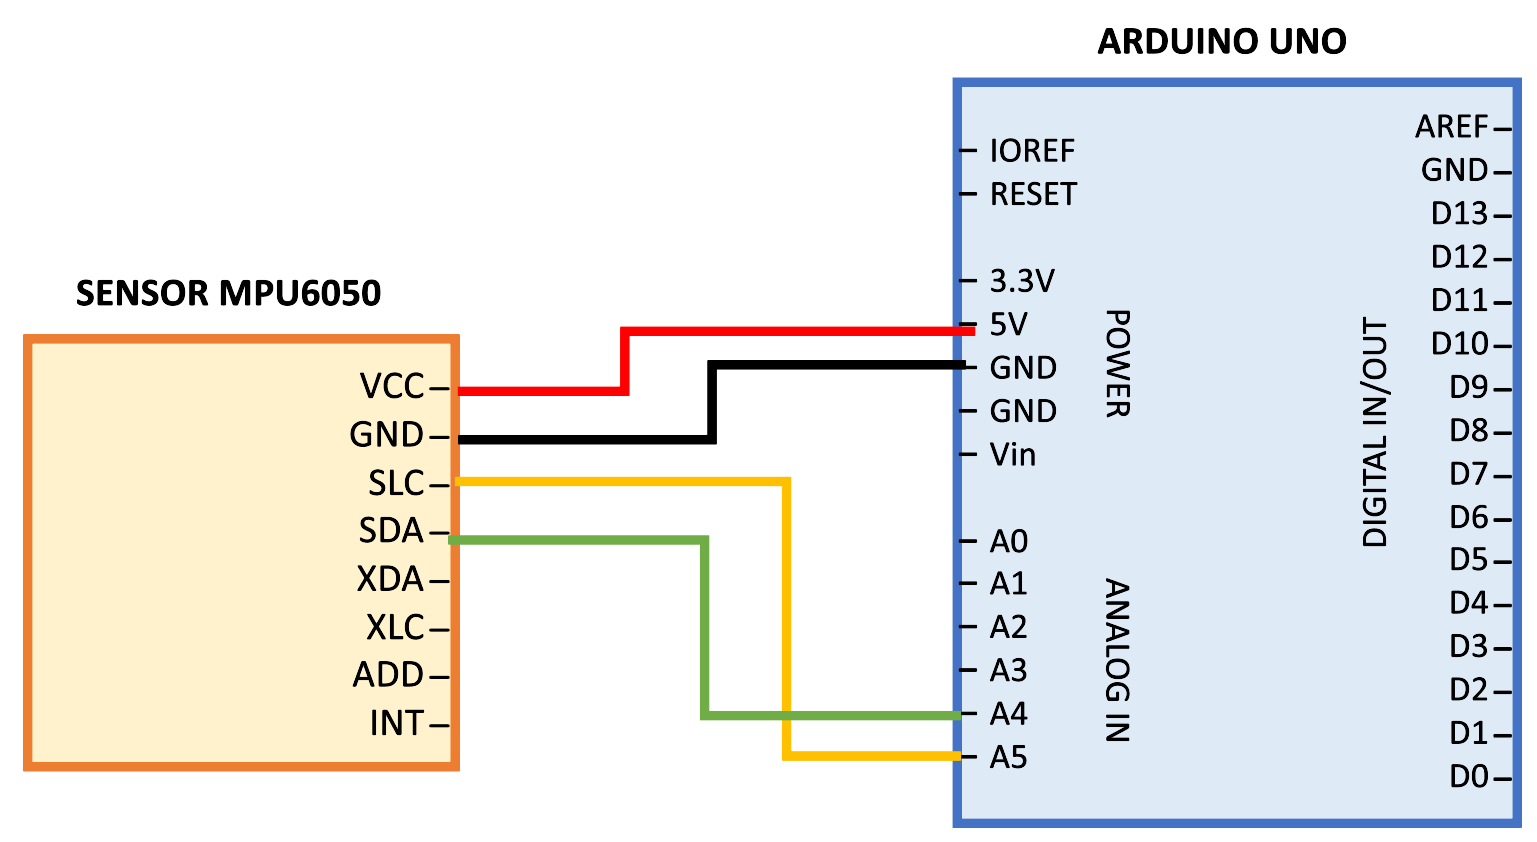
\includegraphics[width=0.5\textwidth]{img/MPU6050.png}
    \caption{Diagrama de las conexiones del módulo MPU6050.}
    \label{fig:MPU6050} % Esta etiqueta es la que permite que se encuentr referenciada en el texto (es muy importante que siempre estén referenciadas en el texto)
\end{figure}

    \item \textbf{Módulo MPU-9250}\cite{MPU9250_1,MPU9250_2}: es un sensor de 9 grados de libertad (9DOF) que permite medir la inclinacion y la aceleración en los 3 ejes. Este módulo incluye un acelerómetro, un giroscopio y un magnetómetro. Al incluir el magenetómetro se elimina la deriva que puede darse tras horas de uso en dispositivos que no tengan este componente. Además, este módulo se acopla mediante bus SPI o por bus I2C. Este sensor necesita una alimentación de entrada de unos 2.4 a 3.6 V, aunque hay algunos módulos que tienen incluido un regulador de voltaje que permite su conexión a un voltaje de 5V. Para programar este módulo es necesaria la librería de Arduino MPU9250\cite{libMPU9250}. 
% Imagen del módulo MPU9250
\begin{figure}[h!]
    \centering
    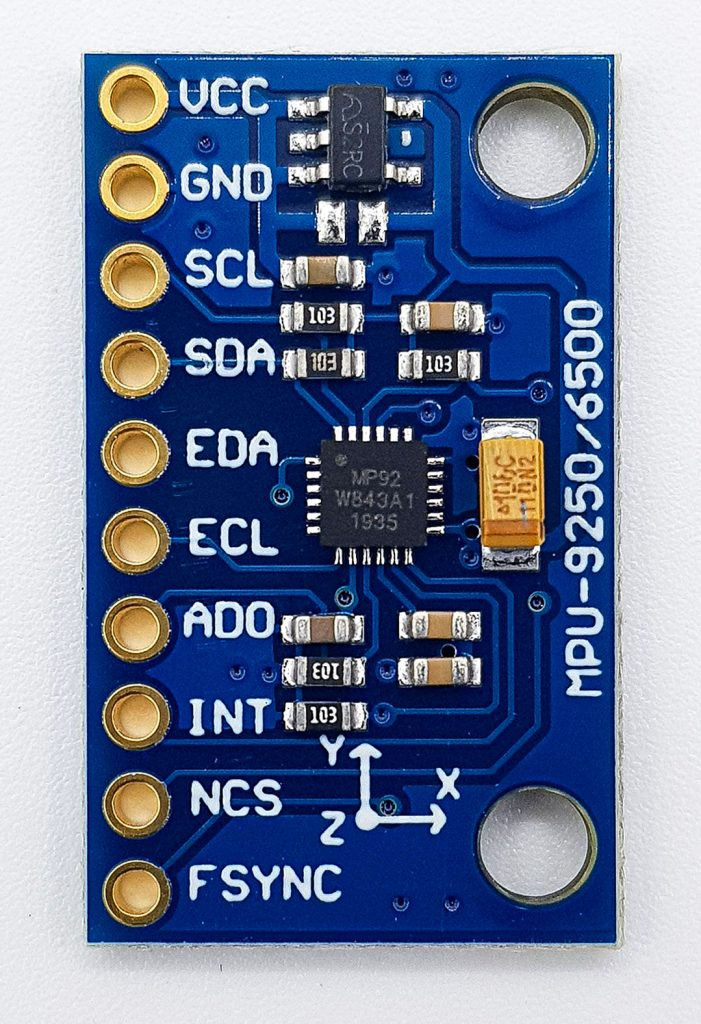
\includegraphics[width=0.15\textwidth]{img/imgMPU9250.jpg}
    \caption{Módulo MPU-9250\cite{imgMPU9250}.}
    \label{fig:imgMPU9250} % Esta etiqueta es la que permite que se encuentr referenciada en el texto (es muy importante que siempre estén referenciadas en el texto)
\end{figure}

% Diagramas del sensor MPU9250
\begin{figure}[h!]
    \centering
    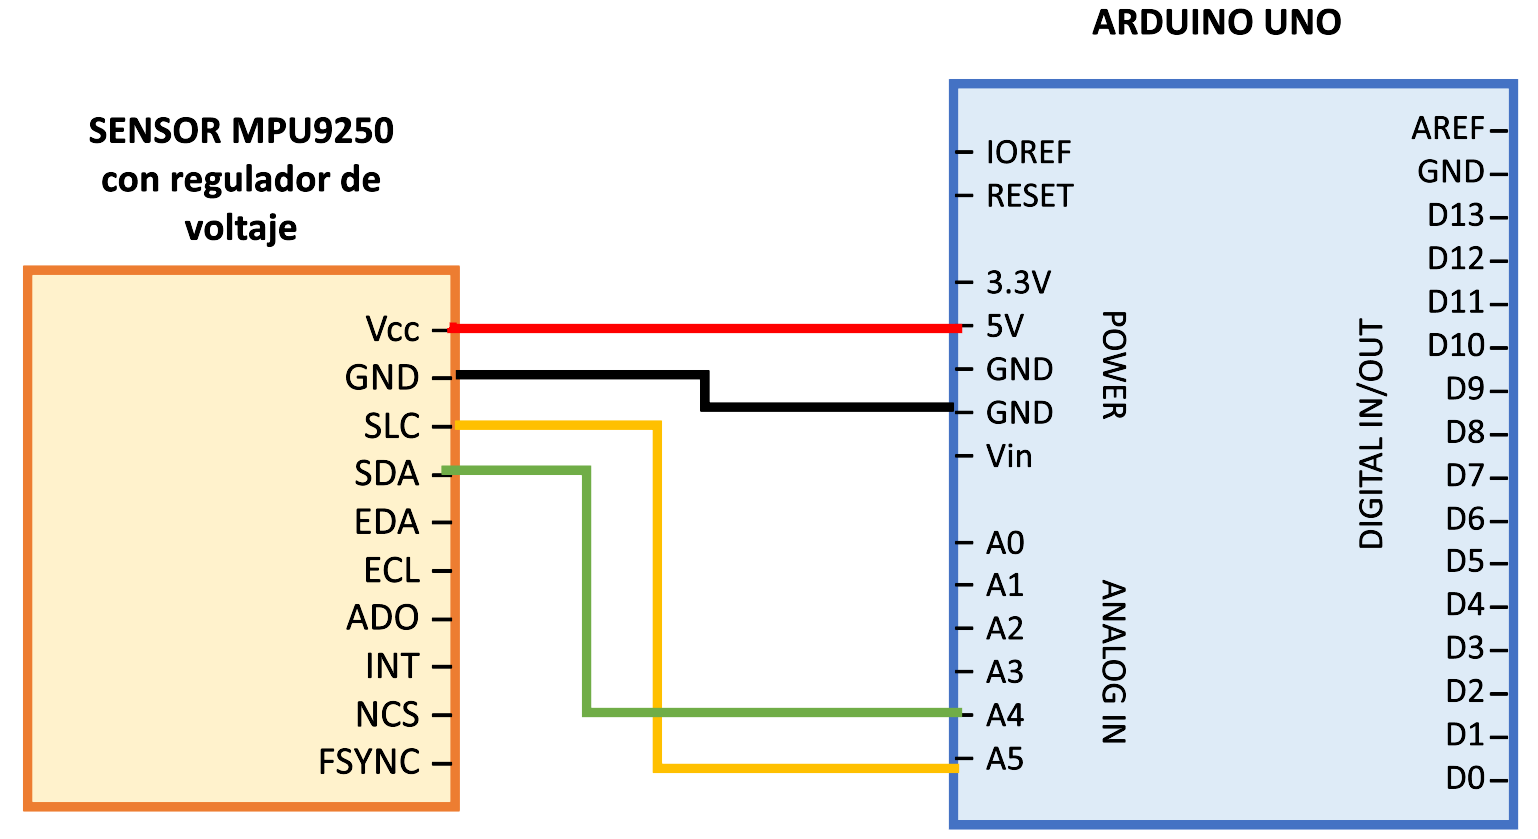
\includegraphics[width=0.5\textwidth]{img/MPU9250Regulador.png}
    \caption{Diagrama del módulo MPU9250 con regulador de voltaje.}
    \label{fig:MPU9250R} % Esta etiqueta es la que permite que se encuentr referenciada en el texto (es muy importante que siempre estén referenciadas en el texto)
\end{figure}
\begin{figure}[h!]
    \centering
    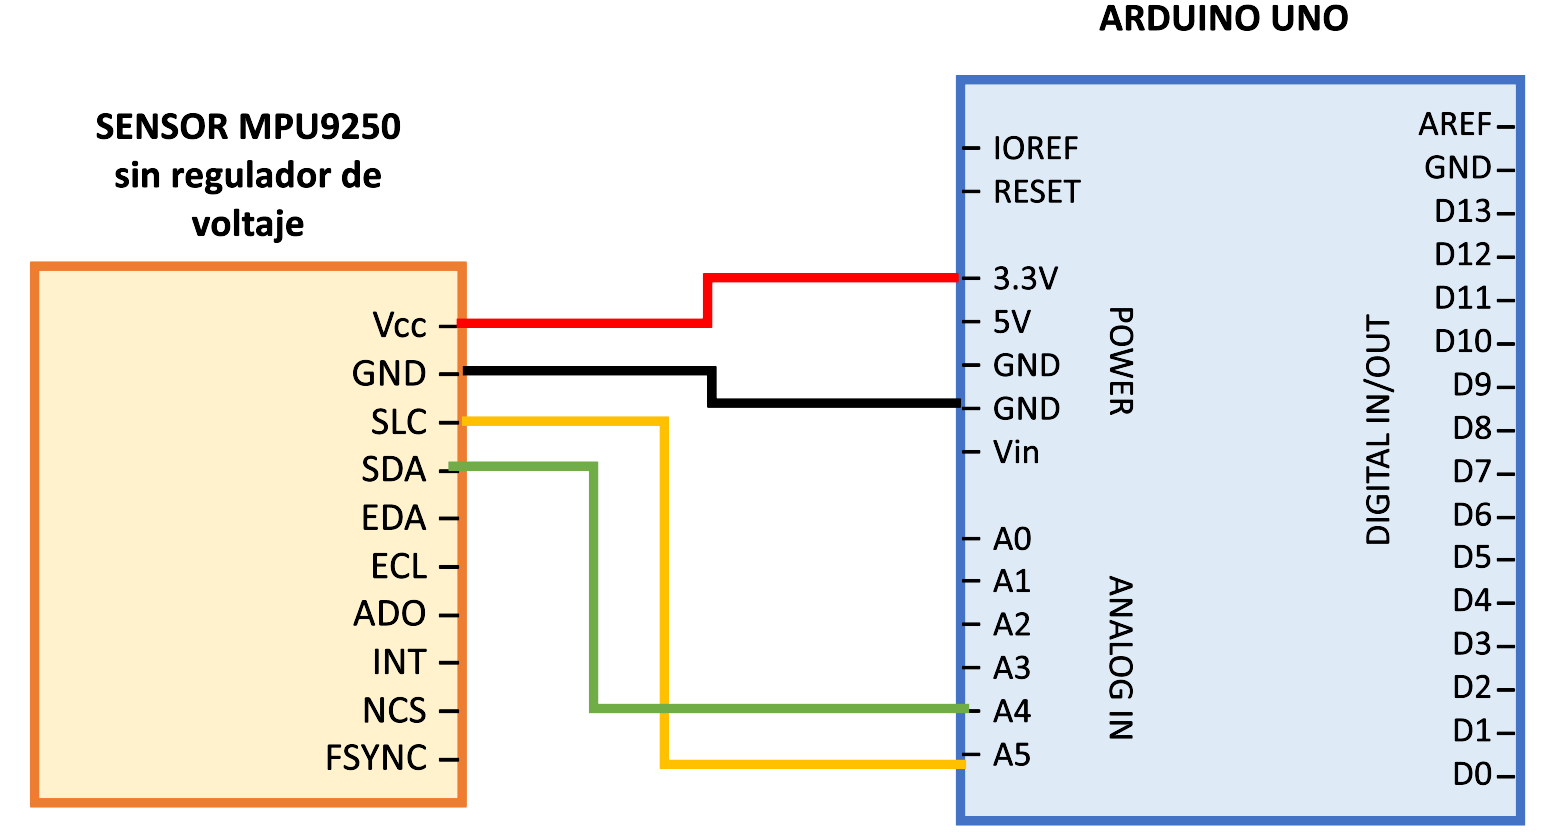
\includegraphics[width=0.5\textwidth]{img/MPU9250SinRegulador.png}
    \caption{Diagrama del módulo MPU9250 sin regulador de voltaje.}
    \label{fig:MPU9250} % Esta etiqueta es la que permite que se encuentr referenciada en el texto (es muy importante que siempre estén referenciadas en el texto)
\end{figure}

\end{itemize}


% ----------------------------------------------------
% Tabla de comparación de sensores
\begin{table}[h!]
\centering
\begin{tabular}{ |m{4cm}|m{8cm}|m{2cm}|  } 
\hline
\cellcolor[HTML]{B9E3F0}\textbf{Módulos} & \cellcolor[HTML]{B9E3F0}\textbf{Características} & \cellcolor[HTML]{B9E3F0}\textbf{Precio}\\

\hline
\cellcolor[HTML]{EFEFEF}\textbf{SCA60C}             & {Mide ángulos de 0-180º y necesita una tensión de entrada de 5V}   & 15-25€\\
\hline
\cellcolor[HTML]{EFEFEF}\textbf{Galgas extensiométricas y módulos HX711}                & {Mide el peso que se ejerce sobre la galga, existen distintas galgas en función del peso a medir y necesita una tensión de entrada de 5V} & 6-15€\\
\hline
\cellcolor[HTML]{EFEFEF}\textbf{ADXL345}                & {Tiene 3 DOF, mide las aceleraciones en los 3 ejes y necesita una tensión de entrada de 2-3.6V} & 3-10€\\
\hline
\cellcolor[HTML]{EFEFEF}\textbf{MPU6050}                & {Tiene 6 DOF, mide aceleraciones y ángulso de rotación en los 3 ejes y necesita una tensión de entrada de 2.4-3.6V} & 5-15€\\
\hline
\cellcolor[HTML]{EFEFEF}\textbf{SW520D}                & {Detecta inclinaciones, es un sensor muy sencillo y actúa como un interruptor. Necesita una tensión de entrada de 5V.} & 0.3-5€\\
\hline
\cellcolor[HTML]{EFEFEF}\textbf{MPU9250}                & {Tiene 9 DOF, mide aceleraciones, ángulos y campos magnéticos en los 3 ejes. Elimina la deriva y necesita una tensión de entrada de 2.4 a 3.6V} & 10-20€\\
\hline
\end{tabular}
\caption{Resumen y comparación de posibles sensores o módulos que se pueden emplear en el proyecto}
\end{table}



Para la realización del prototipo realizado en este proyecto se han seleccionados los módulos SW520D y MPU6050, por sus características, sencillez de uso, precio y disponibilidad. 
\capitulo{4}{Conclusiones}

Desde pequeños hemos oído frases como ``Colócate bien la mochila que te vas a dañar la espalda'', ``Siéntate bien que dentro de unos años te va a doler la espalda'', ``Camina erguido''... Actualmente vivimos en un mundo muy heterogéneo y lleno de tecnologías, ¿por qué seguimos escuchando este tipo de frases?, es sencillo, porque no estamos acostumbrados a mantener una postura correcta. En eso se basa nuestra idea, en crear un dispositivo que nos ayude a acostumbrarnos a una postura correcta para disminuir el daño, además de ayudar a distintos grupos de personas con ciertas patologías que les impide mantener una postura correcta o que se olvidan de mantenerse correctamente erguidos, patologías como puede ser el Parkinson. 

En este trabajo se han estudiado las bases de la postura y del control postural y, su constante modificación a lo largo de la vida de una persona. Asimismo, se han conocido algunas de las opciones que existen en la actualidad para controlar o monitorizar la postura de un usuario, incluyendo algunos dispositivos de diagnóstico de alteraciones posturales y algunos estudios realizados respecto al desarrollo de dispositivos posturales.

Finalmente, gracias a los conocimientos adquiridos durante la búsqueda de información para el proyecto y los conocimientos adquiridos a lo largo de la titulación, se han conseguido dos prototipos sencillos basados en una tecnología de código abierto, Arduino, que permiten mejorar la postura empleando el aprendizaje dinámico basado en biofeedback. 

Como complemento del proyecto se ha ideado un prototipo de interfaz en el que se aúnan las características principales de las aplicaciones existentes de los dispositivos de control postural actuales.


\section{Resumen de resultados.}

Como se ha mencionado previamente, se han creado dos protipos de un dispositivo de control postural. La primera versión del prototipo es la más sencilla, se ha empleado un sensor de inclinación SW520D que actúa como un interruptor. Mientras la persona se encuentre en una buena postura se considerará como apagado y cuando la persona se inclina hacia delante el dispositivo alertará a modo de biofeedback sonoro o vibratorio para que la persona recupere su postura correcta. 

Adicionalmente el primer prototipo incluye un botón de encendido, un led que indica que el dispositivo se encuentra encendido, un zumbador pasivo que emitirá la señal sonora para avisar al usuario y un motor de vibración que emitirá una señal vibratoria. Aunque este último componente no se ha podido conseguir para la demostración.

\textcolor{red}{Añadir imagen del prototipo1 real}

El sensor empleado en la primera versión es muy sensible a vibraciones y por ello se estudiaron otras posibilidades y se realizó un segundo prototipo.

La segunda versión consta de los mismos componentes que la primera versión integrando un botón de calibración y modificando el sensor SW520D\cite{SW520D_1} a un sensor más complejo, el MPU-6050\cite{MPU6050_1,MPU6050_2}, que permite una solución más precisa y amplia, midiendo aceleraciones y rotaciones en los ejes \textit{x},\textit{y} y \textit{z}. El hecho de medir las aceleraciones nos permite calcular por triangulación los ángulos de inclinación, estos ángulos de inclinación son los que han sido empleados para diferenciar entre una buena o una mala postura, si se supera el ángulo umbral se considerará como un postura incorrecta y si se mantiene dentro del umbral se considerará una postura correcta, al igual que en la primera fase si se detecta una mala postura se avisará al usuario mediante biofeedback sonoro o vibratorio. De igual modo, este sensor permitía no solo cumplir con la función de control postural sino que garantizaba la obtención de datos que se pueden emplear para la realización de estadísticas.

\textcolor{red}{Añadir imagen del prototipo2 real}

Para más información y demostraciones de los prototipos se recomienda consultar los anexos correspondientes. Además, en el anexo A se han analizado los costes y la viabilidad legal del proyecto.

Por otro lado, se ha diseñado un prototipo de interfaz de una aplicación que facilite la interacción del usuario con el dispositivo, y que permite un mejor monitoreo y conocimiento de la postura del usuario. En el prototipo de interfaz se plantea no solo las modificaciones de los ajustes del dispositivo, si no que también la visualización de estadísticas de la postura del usuario y la realización de juegos o ejercicios que se incluirán en la aplicación, para el desarrollo musculoesquelético reforzando aquellos músculos relacionados con la postura y facilitando el aprendizaje muscular de una postura natural correcta.

Se puede conocer más información respecto a este prototipo de interfaz en el Anexo F.


\section{Discusión.}
\textcolor{red}{Discusión y análisis de los resultados obtenidos.}

En la primera fase se obtiene el resultado que se esperaba, cumple con la función de control postural, pero no se trata de un sensor muy aceptable frente a vibraciones y no es capaz de registrar datos ya que este dispositivo únicamente trabaja como un interruptor en función de la inclinación en la que se encuentre el sensor, es decir, la persona.

Observando y analizando los fallos encontrados en esta primera versión se realizó el segundo prototipo, la segunda versión, dónde se empleaba el módulo MPU-6050\cite{MPU6050_1,MPU6050_2}, este prototipo ofrece mayor precisión y posibilita recoger datos. Sin embargo este sensor no está pensado para uso prologado, ya que produce deriva.

Este último problema de deriva se podría solucionar con un sensor algo más complejo pero similar al MPU-6050, el MPU-9250\cite{MPU9250_1,MPU9250_2} que incluye un magnetómetro que soluciona este problema. Este último sensor es el qué se habría pensado para una tercera versión pero que no ha sido posible realizar.

% Discusion 
La realización de este tipo de trabajo no solo ha mejorado el control de distintas herramientas como Arduino, Overleaf o GitHub sino que ha proporcionado la comprensión del proceso completo desde la comunicación de una necesidad real hasta la elaboración de un prototipo pasando por la creación de la idea y la selección de los componentes.

Así mismo, este trabajo sirve como ejemplo de las posibilidades y la importancia que ofrece una visita a una asociación, cómo es la Asociacion Parkinson Burgos\cite{ParkinsonBurgos}, dónde se nos ha mostrado el día a día de las personas con esta afectación de la mano de los profesionales, que indicaron necesidades reales y concretas. 

Sin embargo, queda todavía camino que recorrer para obtener un dispositivo de calidad útil, para conseguir este dispositivo sería interesante trabajar en conjunto con asociaciones o profesionales que evalúen la utilidad del dispositivo. Al formar parte de la primera promoción del grado, es la primera vez que se realiza un TFG de estas características, y no ha sido posible integrarse en un laboratorio en concreto para trabajar en conjunto. Cómo se trata de un trabajo de fin de grado muy amplio, existen todavía varios puntos que reforzar. Con todo ello, espero que este trabajo sirva para conocer limitaciones, dificultades y posibles carencias para el futuro.


\section{Aspectos relevantes.}

Se pueden destacar varios aspectos relevantes del proyecto unos relativos a la creación de la idea y otros a la hora de la creación de los prototipos.

\subsection{Selección del tipo de dispositivo}
Tras identificar las características básicas de la postura y el control postural, se ha realizado un estudio de los dispositivos de control postural y de diagnóstico de alteraciones de la postura para poder recoger las características principales que se quieren incluir en nuestro dispositivo. 

A partir de las distintas opciones estudiadas en el estado del arte se decidió que el dispositivo objetivo fuese un dispositivo portátil que controlase la postura de una persona según la inclinación de su postura, para ello se iba emplear aprendizaje dinámico basado en biofeedback vibratorio. Este modelo de biofeedback no solo permite controlar la postura sino que también permite la mejora de la misma a largo plazo. Este aprendizaje de biofeedback se basa en que si el dispositivo detecta una mala postura del usuario se envían avisos de vibración o sonoros para que sea accesible a todas las personas ya tengan alguna discapacidad o no. 

Además, se pretende diseñar una aplicación móvil que reúna las características más relevantes de dispositivos existentes y que interaccione con el dispositivo para que el usuario tenga a su disposición los ajustes del dispositivo, sus estadísticas de mejora en su postura, distintos ejercicios que pueda realizar para mejora de su musculatura troncal y por consiguiente su postura.

Asimismo, la idea era avanzar a modo de Kit teniendo un prototipo base e ir añadiendo componentes para evaluar sus posibilidades y personalizar el dispositivo según las necesidades específicas del usuario.

\subsection{Selección de componentes y diferentes versiones}
Una vez clara la idea base del dispositivo que se pretendía crear, se estudiaron las herramientas y componentes disponibles a nuestra disposición y se seleccionó trabajar con Arduino y su placa UNO R3 ya que se ha empleado en algunas asignaturas del grado. Una vez seleccionado el microprocesador se buscaron componentes compatibles con la plataforma.

Seguidamente, se estudiaron varios sensores que podrían ser útiles para el control postural y se seleccionó en primera opción el sensor SW520D debido a su sencillez y bajo precio.

El primer prototipo se realizó empleando el sensor SW520D y una vez se obtuvo el prototipo se analizó su funcionamiento. Sin ebargo, para que realizara un correcto control postural era necesario colocar el sensor en un determinado ángulo por lo que sería necesario crear una carcasa donde encaje el sensor en ese ángulo o mantener el dispositivo con algún tipo de control de nivel. Por otro lado, este primer sensor es muy sensible a vibraciones por lo que no es de gran precisión y no proporciona datos exactos, por ello, se decidió seguir con el siguiente prototipo.

Para el segundo prototipo se decidió emplear el MPU-6050 por su precisión y precio. Este sensor incluye un acelerómetro y un giroscopio que permite conocer en todo momento aceleraciones y rotaciones y, en consecuente, inclinaciones en los distintos ejes. Una vez creado el nuevo prototipo se implementó un programa en el que se incluía el águlo umbral para considerar buena postura y el tiempo de espera para avisar de una postura incorrecta y de esta forma monitorizar la misma. Este prototipo permite recopilar las distintas aceleraciones y rotaciones y por lo tanto estos datos se podrían emplear para realizar distintas estadísticas que se puedan mostrar al usuario.

No obstante, este último prototipo requiere de calibración cada vez que se emplea el dispositivo para poder mantener la buena precisión y, para la calibración el dispositivo no se debe mover y debe estar sobre una superficie plana, por lo que se ha tenido que crear una base de sustentación. Esta base se ha creado con material reciclado de cartón.

Asimismo, el módulo MPU-6050 tiene un problema de deriva por lo que no es apto para uso prolongado. Para solucionar este problema se puede emplear el módulo MPU-9250 que sería el sensor una nuestra tercera versión, que no se ha podido realizar por falta de tiempo.





%\capitulo{5}{Aspectos relevantes del desarrollo del proyecto}

\capitulo{4}{Lineas de trabajo futuras}


Este capítulo debería ser informe crítico indicando cómo se puede mejorar el proyecto, o cómo se puede continuar trabajando en la línea del proyecto realizado.

En este trabaja únicamente se ha realizado un prototipo y será necesario en el futuro, crear la aplicación, el dispositivo de forma más robusta, corregir errores que han surgido, crear juegos o ejercicios que se podrán realizar con el dispositivo para así mejorar la musculatura y la postura de los usuarios que utilicen el dispositivo.

Se puede mejorar el proyecto profundizando más en las posibilidades de los sensores de presión y otros de los dispositivos incuidos en el estado del arte y los posibles usos que se pueden realizar con  otros productos como mallas o calcetines inteligentes.

% -----------------BIBLIOGRAFÍA-------------------
%\bibliographystyle{plain} % Sin URL con números
%\bibliography{bibliografia}

% Si se salen de los márgenes las referencias:
%\newgeometry{left= 3cm, right = 3cm}
\printbibliography[]



\end{document}
